\documentclass[12pt, a4paper]{ujreport} % a4jでもOKっぽい

%% ----- packages ----- %%
% --- 図表 --- %
\usepackage{plautopatch}
\usepackage[dvipdfmx]{graphicx, xcolor, pict2e} % geometory: 余白設定 graphicx: 画像挿入 xcolor: 文字の色付け pict2e: 図が描ける
\usepackage{here} % 図の配置を指定できる
\usepackage{float} % here と同じらしい
\usepackage{longtable} % 表
\usepackage{colortbl} % 表に色を付ける
\usepackage{tabularx} % 表組みの設定
\usepackage{enumerate} % 番号付き箇条書き
\usepackage{lscape} % 図表回転
\usepackage{multirow} % 表のセルに連続して同じ値を書くときにまとめて書ける(行)
\usepackage{diagbox} % 表ヘッダ作成
\usepackage{multicol} % 表のセルに連続して同じ値を書くときにまとめて書ける(列)
\usepackage{wrapfig} % 図と文章を並べて書ける
\usepackage{hhline}
% \usepackage{graphicx}

% --- 文字 --- %
\usepackage{bm} % 太字の斜体
\usepackage{underscore} % アンダーバー"_"を表示できる
\usepackage{plext} % 縦書きを横書きで書ける
\usepackage{fancyhdr} % ヘッダとフッタを編集できる
\usepackage{ulem} % 下線が引ける
\usepackage{cite} % 参考文献リスト"bibitem"の参照
\usepackage{times} % フォント "times" に指定
\usepackage{mathptmx} % 数式も含めてフォント "times" に指定
\usepackage{amsmath,amssymb,amsfonts} % 数式をきれいに書ける。amsfontsはフォントを指定しているが、mathptmxでフォント指定されているため、機能していない。
\usepackage{algorithmic} % アルゴリズム(疑似コード)を書ける
\usepackage{textcomp} % 特殊文字を書ける
\usepackage{comment} % コメントアウト
\usepackage{url} % url挿入
%\usepackage[ipaex]{pxchfon} %文書内の和文フォントの指定(ipaexフォントが指定されている, 無くても大丈夫そう)
%\usepackage[uplatex, deluxe]{otf}

%% --- ページ設定 --- %%
% \usepackage[top=30truemm,bottom=30truemm,left=30truemm,right=20truemm]{geometry} % 余白設定

% (すぐ上の行を使わないとき用)
\makeatletter
% \setlength{\voffset}{0.5truecm} % old 上余白 (1)
% \setlength{\oddsidemargin}{7.0truemm} % old 左余白 (3): 25.4mm + 7.0mm = 32.4mm
\setlength{\oddsidemargin}{4.6truemm} % 左余白: 25.4mm + 4.6mm = 30mm, 13pt
% \setlength{\evensidemargin}{-5.5truemm} % old 偶数頁左余白 (3): 25.4 - 5.5mm = 19.9mm, jreportなので不要?
% \setlength{\topmargin}{-1truecm} % old (4)
\setlength{\topmargin}{-23pt} % -12pt+(-11pt) = -23pt, 8.1mm (4)
% \setlength{\headsep}{2truecm} % old 上余白 (6)
\setlength{\headsep}{25pt} % 8.81mm, 12pt+14pt=25pt (6), 上余白30mmになるように設定した
% \setlength{\textheight}{22truecm} % old (7)
\setlength{\textheight}{672pt} % 845pt-85pt*2, 237truemm (7), 下余白30mmになるように設定した
% \setlength{\textwidth}{15truecm} % old (8)
\setlength{\textwidth}{441pt} % (8) 155truemm, 右余白25mmになるように設定した
% \setlength{\footskip}{25truemm} % old (11)
\setlength{\footskip}{30pt} % 10.5pt+19.5pt=30pt, 10.6mm(11), ページ数の位置
% 1pt = 0.35mm
\makeatother


%% ----- main ----- %%
\begin{document}

\pagenumbering{roman}
\title{
曖昧な話し言葉判別にむけた教師ラベル作成支援に関する研究\\
Research on Construction Support of Teacher Labels Toward the Discrimination of Ambiguous Spoken Word
}
\author{
指導教員: 小松川 浩 \\
公立千歳科学技術大学 理工学部 \\
理工学専攻 博士前期課程2年 \\
小松川・山川・深町研究室 \\
令和5年度 \\
m2220180 新井田 響}
\date{\today}
\maketitle
\tableofcontents
%\thispagestyle{empty}

\chapter{序論\label{c1}}
\pagenumbering{arabic}

\section{背景}
現在,レポートや論文の書き方をはじめとする文章作成技法に関する講義が開講され,様々な教育機関において文章作成能力の向上が求められている.一方で,文章作成技法に関する講義の指導方法は各教育機関や教員によって異なり,模範となる指導方法は確立されていない.これは大学についても同様である.

レポートや論文は,学術的文章に適した表現で記述することが求められる.しかし,学術表現に従ったレポートを作成できない学生が多く存在し,特に,文章中に話しことばが混在することが問題視されている.これらの課題に対し,本研究チームは,話しことばの情報を集約したデータベースを活用し,話しことばカテゴリに基づく添削を行う大学初年次向け文章添削システム「話しことばチェッカー」に関する研究を行ってきた.

ある表現が話しことばであるか書きことばであるかが採点者によって解釈が分かれる可能性のある曖昧な表現が存在し、文章作成において一貫した指導が難しいとされている.その要因として、あいまいな表現が,話しことばであるか書きことばであるかが文脈の中でどのように用いられているかによって決まる表現が存在することが挙げられる.一方で本システムでは、ルールベースのアルゴリズムに基づく話しことば検出を行うため、正しい検出結果を示すことができないという課題がある.以上のような文脈によって話しことばとも書きことばともとれる表現が存在することがわかっており、本研究チームではこの表現を「グレーゾーン」と定義している.

近年発達してきた機械学習の手法を用いることによって文章内の単語の位置関係以外にも,文脈を考慮した単語の位置関係の把握も行えるようになってきた.また,インターネットの発展とともに,文章や画像のデータセットを無償で利用できることも可能になってきている.先行研究では,グレーゾーンを含む文章が主観的であれば,そのグレーゾーンは話しことば,客観的であれば書きことばに分類できるという仮定のもと,インターネットから収集したグレーゾーンを含む文章を学習させ,グレーゾーンの判別が可能な機械学習モデルの構築を試みた.

しかし,学習データや検証データの確保については,手作業による事例収集やラベル付けについても,専門家が個々のデータを見て判断する必要があるなどといった問題がある.すべてのグレーゾーンの判別が可能な機械学習モデルを構築するために各々のグレーゾーン用のデータセットを作成することは現実的ではない.

\section{目的}
機械学習によるグレーゾーンの話しことば判定を行うためには,機械学習に用いるデータの確保は必要不可欠である.しかし,グレーゾーンを含む文章を大量に収集することは困難である.また,すべてのグレーゾーンについて事例を収集し,そのグレーゾーンが話しことばに分類されるか書きことばに分類されるかのラベリングは専門家にとって時間や労力の観点で大きな負担となり得る.そこで本研究では,機械学習モデル構築で必要になるデータ収集やラベル付けの効率化について検討し,さらにLLMによる文章生成を用いたデータ作成支援,データ収集の効率化の方策についての検討を通し,AIとルールベースを組み合わせた「AI話しことばチェッカー」構築の負担軽減を図る.

\section{構成}
本論文の構成について述べる.
第2章では,本研究チームで開発・運用しているシステムである「話しことばチェッカー」に関する先行研究について述べる.
第3章では,話しことばチェッカーの紹介と,日本語教育の専門家らでも話しことばか書きことばかの判断が分かれる表現である「グレーゾーン」について述べる.
第4章では,本研究に関わる機械学習手法について述べる.
第5章では,機械学習モデル構築に関する課題について述べる.
第6章では,LLMを用いたグレーゾーン表現の主観客観判定に関する検証について述べる.
第7章では,LLMを用いた話しことば検出について述べる.
第8章では,まとめと今後の展望について述べる. % 背景目的
\chapter{先行研究と本研究の位置づけ\label{c2}}

\section{話しことばチェッカーの開発と実証評価 \label{c2s1}}
「話しことばチェッカーの開発と実証評価」は本研究チームの山下による研究である.学生が提出したレポートに含まれる話しことばの個数を,話しことばチェッカーによる判定を受ける前後でどの程度変化したかの調査が行われている.今後の課題として,システムの誤検出およびパターンマッチによる検出では判断しきれない表現への対応が挙げられており,機械学習を活用した文脈判断による話しことば検出の必要があると述べられている.パターンマッチによる検出では判断しきれない曖昧な表現の例として「~てしまう」が挙げられ,その表現が出現する文章の主語が一人称であれば主観的,三人称であれば客観的となり,機械学習を用いることでそれぞれ話しことば,書きことばに分類できる可能性が示唆されている.

\section{学生のレポートにおける話し言葉とその出現傾向 \label{c2s2}}
「学生のレポートにおける話し言葉とその出現傾向」は本研究チームの山下による研究である.レポートの書き方に関する書籍で取り扱われる話しことばについてまとめ,「学術文章作法I」で提出された学生のレポートから抽出した話しことばについて分析している.ある表現について,話しことばか書きことばかの判断が添削者により異なる表現が存在することや,話しことばをどのように書きことばに書き改めるべきかの判断が難しい事例が存在することなどが示されている.具体例として,「~から」「~ので」について,それぞれを「~ために」に書き改めるよう指示している場合や,「~から」を「~ので」への置き換えを許容する場合が存在する.本研究チームでは,文章に含まれる話しことばを検出する Web システムである話しことばチェッカーの研究および開発を行っているが,このような曖昧な表現について柔軟に対応ができないという課題がある.

\section{AI話しことばチェッカーを想定した機械学習モデリングに関する研究 \label{c2s3}}
「AI話しことばチェッカーを想定した機械学習モデリングに関する研究」\cite{ai-checker}は川越による研究である.\ref{c2s1}節で示唆されたグレーゾーンを含む文章の主語が一人称であれば主観的,三人称であれば客観的となり,機械学習を用いてそれぞれ話しことば,書きことばに分類できるという観点に基づき,本研究チームが定義したグレーゾーンの一つである「てしまう」に着目し,機械学習が有効かを調査した.機械学習モデルであるBERTを用い,Amazonレビュー文章を主観的な文章,論文データセットを客観的な文章と定めたデータセットでファインチューニングを行った.ファインチューニング後のモデルの正解率は77\%となり,グレーゾーンの話しことば・書きことばの判別に特化したAI話しことばチェッカーの実現可能性が示唆された.一方で,今回は「てしまう」のみの結果であり,グレーゾーンは他にも指定された語句が存在することから,「てしまう」以外のグレーゾーン表現を含む文章の主観・客観を判定できるより汎用的なモデルの構築を課題として残している.

% 日本語の話しことばや書きことばは,文章内の単語や,単語同士の関
\section{本研究の位置づけ}
グレーゾーンは「てしまう」以外にも存在している.現状では「てしまう」以外のグレーゾーンも判定できる機械学習モデル構築には着手していないが,機械学習モデル構築までの手順は先行研究と同様にして行うことで実現できることが明らかになっている.グレーゾーンは今後も種類が増えていくことが予想されるため,継続的なデータの確保を考慮することが必要となる.本研究では,AI話しことばチェッカー実現に向けて起こるコストや負担の軽減について検討し,どのような手法が有効かを考察する.
 % 先行研究位置づけ
\chapter{話しことばチェッカーとグレーゾーン\label{c3}}

% 話しことばチェッカー関連

\section{本研究における話しことばの定義 \label{c3s1}}
本研究チームにおける「話しことば」の定義は,大学初年次の学生が自らレポート推敲が行えることが望ましい非学術的な表現と定義されている.ただし,本研究チームにおいての話しことばは,会話による話し言葉ではなく,レポートや論文などの文章に現れる「書かれた話し言葉」を指す.

\section{話しことばカテゴリ \label{c3s2}}
これまでの研究により,話しことばには,単語そのものが話しことばである表現や,単語の位置関係,例えばある単語の直前にある単語との組み合わせによって話しことばと判断される表現が存在することがわかっている.これらの表現に対し,本研究チームでは「話しことばカテゴリ」と定義している.カテゴリは,表\ref{RJCS-category}に示すように,前述のような単語の位置関係や品詞などに応じて5つに分類される.

\begin{table}[H]
\centering
\caption{話しことばカテゴリ}
\begin{tabular}{|c|l|l|l|}
\hline
\multicolumn{1}{|c|}{番号} & \multicolumn{1}{c|}{名称} & \multicolumn{1}{c|}{説明} & \multicolumn{1}{c|}{例} \\ \hline
1 & INDEPENDENCE & 対象の単語がある           & \begin{tabular}[c]{@{}l@{}}当たり前、\\あんまり\end{tabular} \\ \hline
2 & PREFIX       & \begin{tabular}[c]{@{}l@{}}対象の単語およびその直前に\\ 特定の品詞の単語がある\end{tabular} & \begin{tabular}[c]{@{}l@{}}名詞+して、\\動詞+して\end{tabular} \\ \hline
3 & SUFFIX       & \begin{tabular}[c]{@{}l@{}}品詞の組み合わせを必要とせず、\\なおかつ複数の単語から成り立つ\end{tabular} & \begin{tabular}[c]{@{}l@{}}くせ+に、\\ かも+しれ+ない\end{tabular} \\ \hline
4 & COLLOCATION  & \begin{tabular}[c]{@{}l@{}}対象の単語およびその単語と\\同じ文章に特定の単語がある\end{tabular} & \begin{tabular}[c]{@{}l@{}}一番+形容詞\\ どうしても+たい \end{tabular} \\ \hline
5 & OTHER   & \begin{tabular}[c]{@{}l@{}}文法的誤り、若者的な言葉遣いなど、\\上記4つ以外に当てはまるもの\end{tabular}  & 全然+違う \\ \hline
\end{tabular}
\label{RJCS-category}
\end{table}

\section{話しことば事例集 \label{c3s3}}
本研究チームが取り扱う話しことばは,日本語教育のエキスパートによる分類によって定められている\cite{checker-dthesis}.分類する際の基準は,大学生向けのレポートの書き方について書かれた関連書籍で示されていることである.過去の研究では,前述の基準で示された話しことばや,初年度教育の講義で学生が作成したレポートなどから話しことばの抽出を行い,話しことば事例集としてまとめた.エキスパートが話しことばを抽出する際に用いた関連書籍の一覧を表\ref{spoken-book}に示す.

\begin{table}[H]
\centering
\caption{「レポートの書き方」関連書籍一覧}
\begin{tabular}{|l|}
\hline
\begin{tabular}[l]{@{}l@{}}創価大学学士課程教育機構(2017)『レポート作成の手引き 2017 年度版』\end{tabular} \\ \hline
\begin{tabular}[l]{@{}l@{}}秋岡伸彦(2007)『文章表現テキスト』東京農業大学出版会\end{tabular}  \\ \hline
\begin{tabular}[l]{@{}l@{}}石黒圭(2012)『この1冊できちんと書ける!論文・レポートの基本』\\ 日本実業出版社\end{tabular}  \\ \hline
\begin{tabular}[l]{@{}l@{}}石坂春秋(2003)『レポート・論文・プレゼンスキルズ』くろしお出版\end{tabular}  \\ \hline
\begin{tabular}[l]{@{}l@{}}井下千以子(2014)『思考を鍛えるレポート・論文作成法〔第 2 版〕』\\慶応義塾大学出版会\end{tabular}  \\ \hline
\begin{tabular}[l]{@{}l@{}}上戸理恵・遠藤郁子・神田由美子・羽矢みずき・藤田和美・与那覇惠子(2016)\end{tabular}  \\ \hline
\begin{tabular}[l]{@{}l@{}}『新編マスター日本語表現〔第 2 版〕』ひつじ書房\end{tabular}  \\ \hline
\begin{tabular}[l]{@{}l@{}}大島弥生・池田玲子・大場理恵子・加納なおみ・高橋淑郎・岩田夏穂(2014)\end{tabular}  \\ \hline
\begin{tabular}[l]{@{}l@{}}『ピアで学ぶ大学生の日本語表現〔第 2 版〕』ひつじ書房\end{tabular}  \\ \hline
\begin{tabular}[l]{@{}l@{}}石井一成著(2011)『ゼロからわかる大学生のためのレポート・論文の書き方』\\ナツメ社\end{tabular}  \\ \hline
\begin{tabular}[l]{@{}l@{}}長尾佳代子・村上昌考(2015)『大学1年生のための日本語技法』ナカニシヤ出版\end{tabular}  \\ \hline
\begin{tabular}[l]{@{}l@{}}銅直信子・坂東実子(2013)『大学生のための文章表現\&口頭発表練習帳』\\ 図書刊行会\end{tabular}  \\ \hline
\begin{tabular}[l]{@{}l@{}}森下稔・久保田英助・鴨川明子編(2010)『新版 理工系学生のための日本語表現法』\\東信堂\end{tabular}  \\ \hline
\begin{tabular}[l]{@{}l@{}}菊田千春・北林利治(2006)『大学生のための論理的に書き、プレゼンする技術』\\ 東洋経済新報社\end{tabular}  \\ \hline
\begin{tabular}[l]{@{}l@{}}伊藤義之(2003)『はじめてのレポート レポート作成のための 55 のステップ』\\ 嵯峨野書院\end{tabular} \\ \hline
\end{tabular}
\label{spoken-book}
\end{table}

% 使用箇所: c3s3

話しことば事例集では,抽出した話しことばに対し,話しことばカテゴリ,その表現が話しことばである理由,書きことばへの修正例を追加情報として付与している.

\begin{table}[H]
\centering
\caption{話しことば事例集から抜粋}
\small % \footnotesize
\begin{tabular}{|c|c|l|l|}
\hline
\multicolumn{1}{|c|}{話しことば} & \multicolumn{1}{c|}{カテゴリ} & \multicolumn{1}{c|}{原文} & \multicolumn{1}{c|}{修正例} \\ \hline
あいにく & INDEPENDENCE & \begin{tabular}[c]{@{}l@{}} 陸上種目の初日は\\あいにくの雨だった. \end{tabular}              & \begin{tabular}[c]{@{}l@{}}陸上種目の初日は\\雨だった.\end{tabular} \\ \hline
当たり前 & INDEPENDENCE & \begin{tabular}[c]{@{}l@{}}水道の水が飲めるのは\\日本だけでは当たり前の\\ことである.\end{tabular} & \begin{tabular}[c]{@{}l@{}}水道の水が飲めるのは\\日本だけでは当然の\\ことである.\end{tabular} \\ \hline
し      & PREFIX       & \begin{tabular}[c]{@{}l@{}}営業時間を退縮すれば,\\客が減るし売り上げも\\減る.\end{tabular}       & \begin{tabular}[c]{@{}l@{}}営業時間を退縮すれば,\\客が減り売り上げも\\減る.\end{tabular} \\ \hline
てる    & PREFIX       & \begin{tabular}[c]{@{}l@{}}犯罪に巻き込まれる危\\険性が指摘されてる.\end{tabular}               & \begin{tabular}[c]{@{}l@{}}犯罪に巻き込まれる危\\険性が指摘されている. \end{tabular} \\ \hline
くせに   & SUFFIX      & \begin{tabular}[c]{@{}l@{}}社会人のくせに名刺の\\渡し方も知らない.\end{tabular}                 & \begin{tabular}[c]{@{}l@{}}社会人でありながら\\名刺の渡し方も知らない. \end{tabular}\\ \hline
てて    & SUFFIX       & \begin{tabular}[c]{@{}l@{}}仕事をしてても SNS \\のこと気になる状態を \\SNS 中毒という.\end{tabular} & \begin{tabular}[c]{@{}l@{}}仕事をしていても SNS \\のことが気になる状態を \\SNS 中毒という.\end{tabular} \\ \hline
一番    & COLLOCATION  & \begin{tabular}[c]{@{}l@{}}家族には一番の味方で\\あってほしいと願うものだ.\end{tabular} & \begin{tabular}[c]{@{}l@{}}家族には最大の味方で\\あってほしいと願うものだ.\end{tabular} \\ \hline
一番に   & OTHER        & \begin{tabular}[c]{@{}l@{}}一番に解決しなければ\\ならない.\end{tabular} & \begin{tabular}[c]{@{}l@{}}初めに解決しなければ\\ならない.\end{tabular} \\ \hline


\end{tabular}
\label{spoken-ex}
\end{table}











\section{話しことばチェッカー \label{c3s4}}
本研究チームで研究および開発・保守を行っている話しことばチェッカーは,文章中に含まれる話しことばを検出し,書きことばへの修正例を提示し,学生自身による推敲をサポートするWebシステムである.

\begin{figure}[H]
	\centering
 	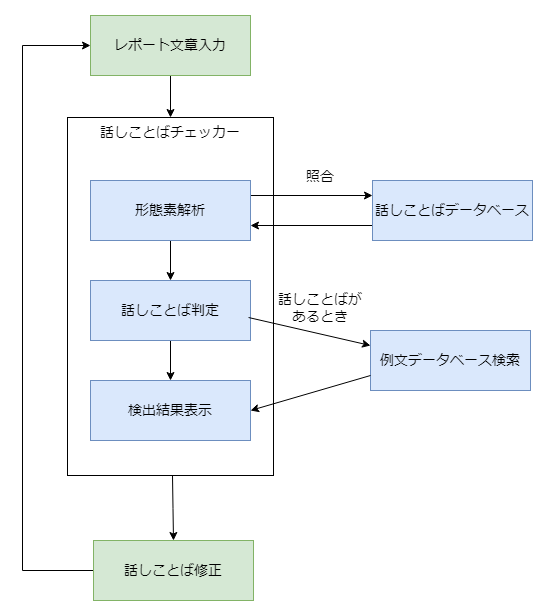
\includegraphics[width=120mm]{image/checker-flow.png}
	\caption{話しことばチェッカーの利用フロー}
	\label{checkerss-flow}
\end{figure}

\begin{figure}[H] % 別の画像貼る
	\centering
 	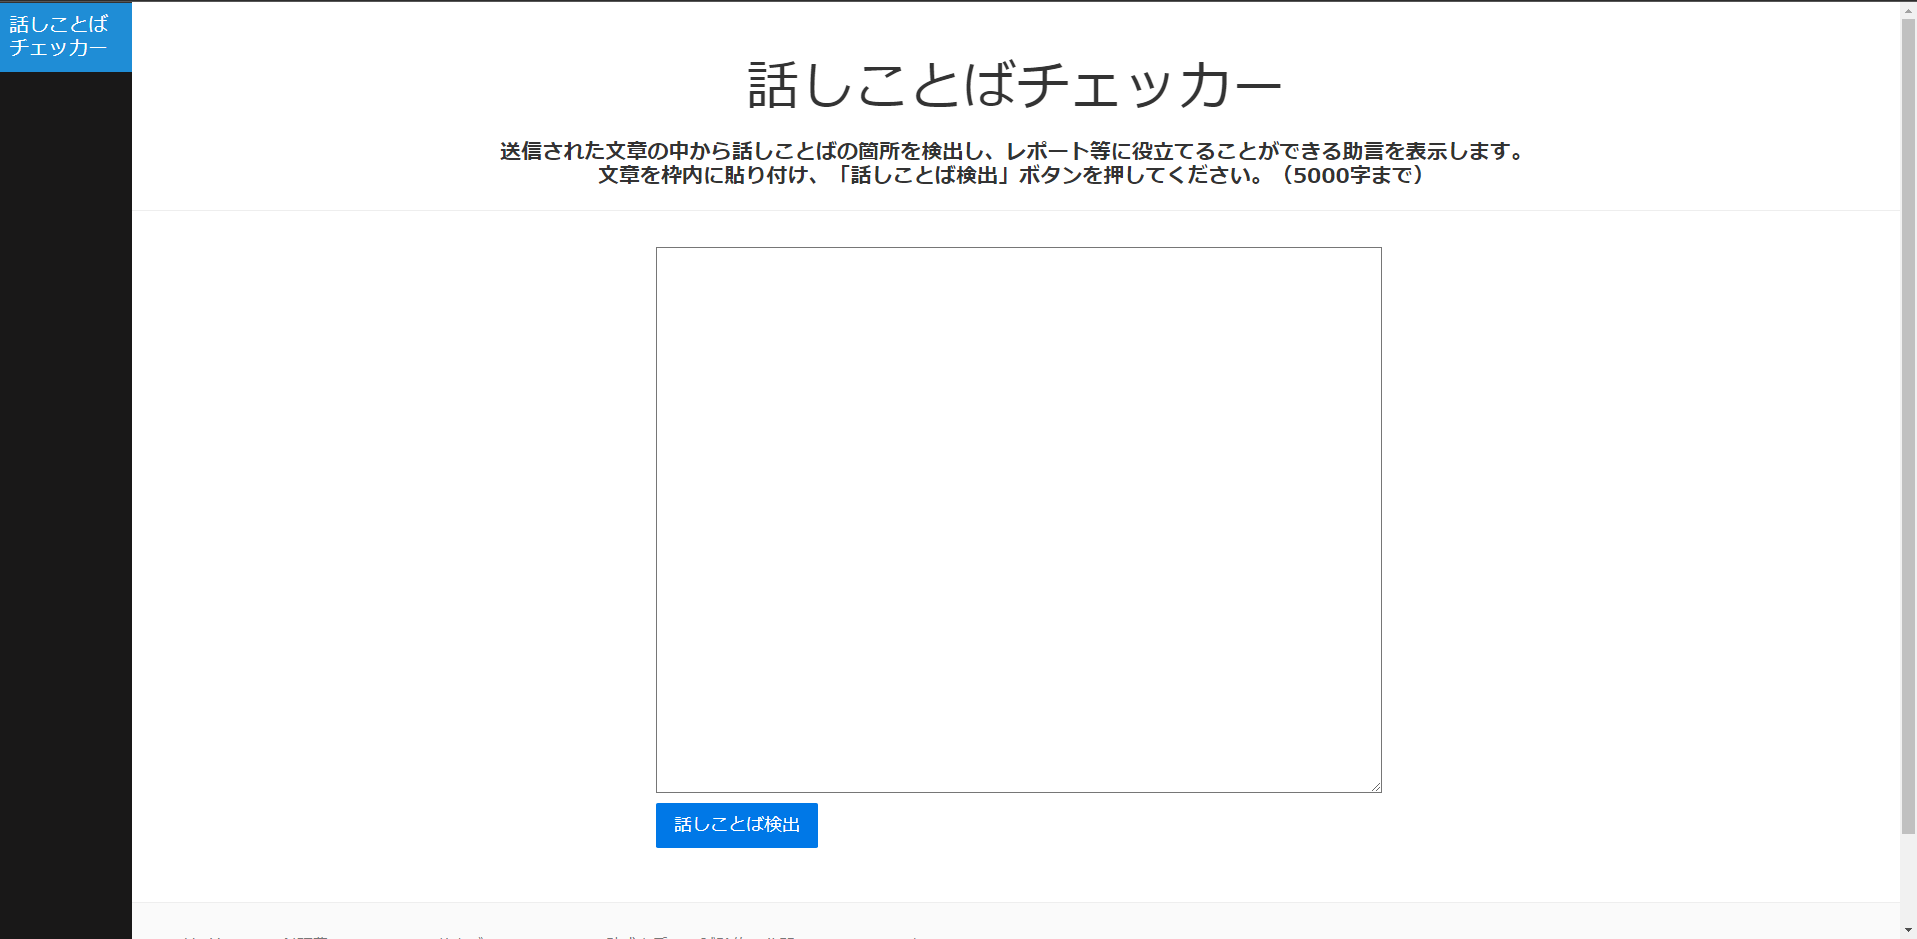
\includegraphics[width=150mm]{image/checkerss-plain.png}
	\caption{話しことばチェッカーの入力画面}
	\label{checkerss-plain}
\end{figure}

レポートなどの文章を入力し提出することで,文章中の話しことばの箇所が色付けされる.画面上で,色付けされた箇所にマウスを合わせると,書きことばへの修正例およびコメントといった推敲のための補足情報が確認できる.実際の利用画面を図\ref{checkerss-result},図\ref{checkerss-popout}に示す.

\begin{figure}[H]
	\centering
 	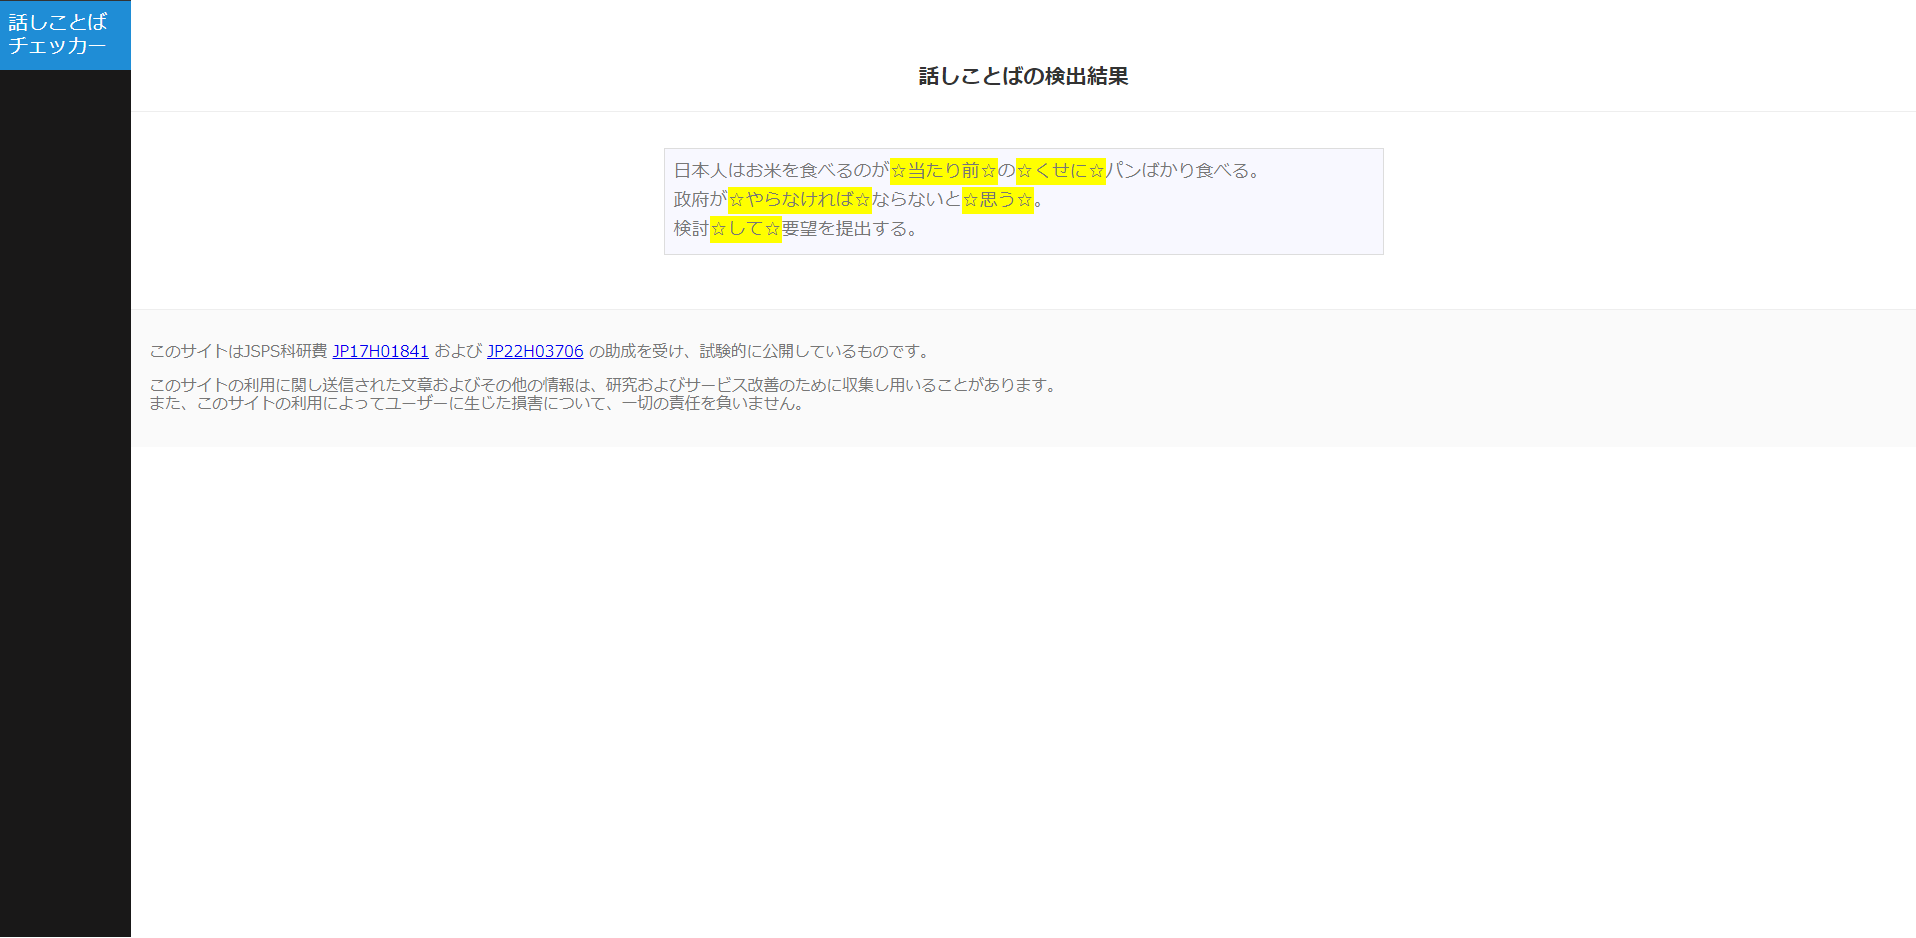
\includegraphics[width=150mm]{image/checkerss-result.png}
	\caption{話しことばチェッカーの話しことば検出画面}
	\label{checkerss-result}
\end{figure}

\begin{figure}[H]
	\centering
 	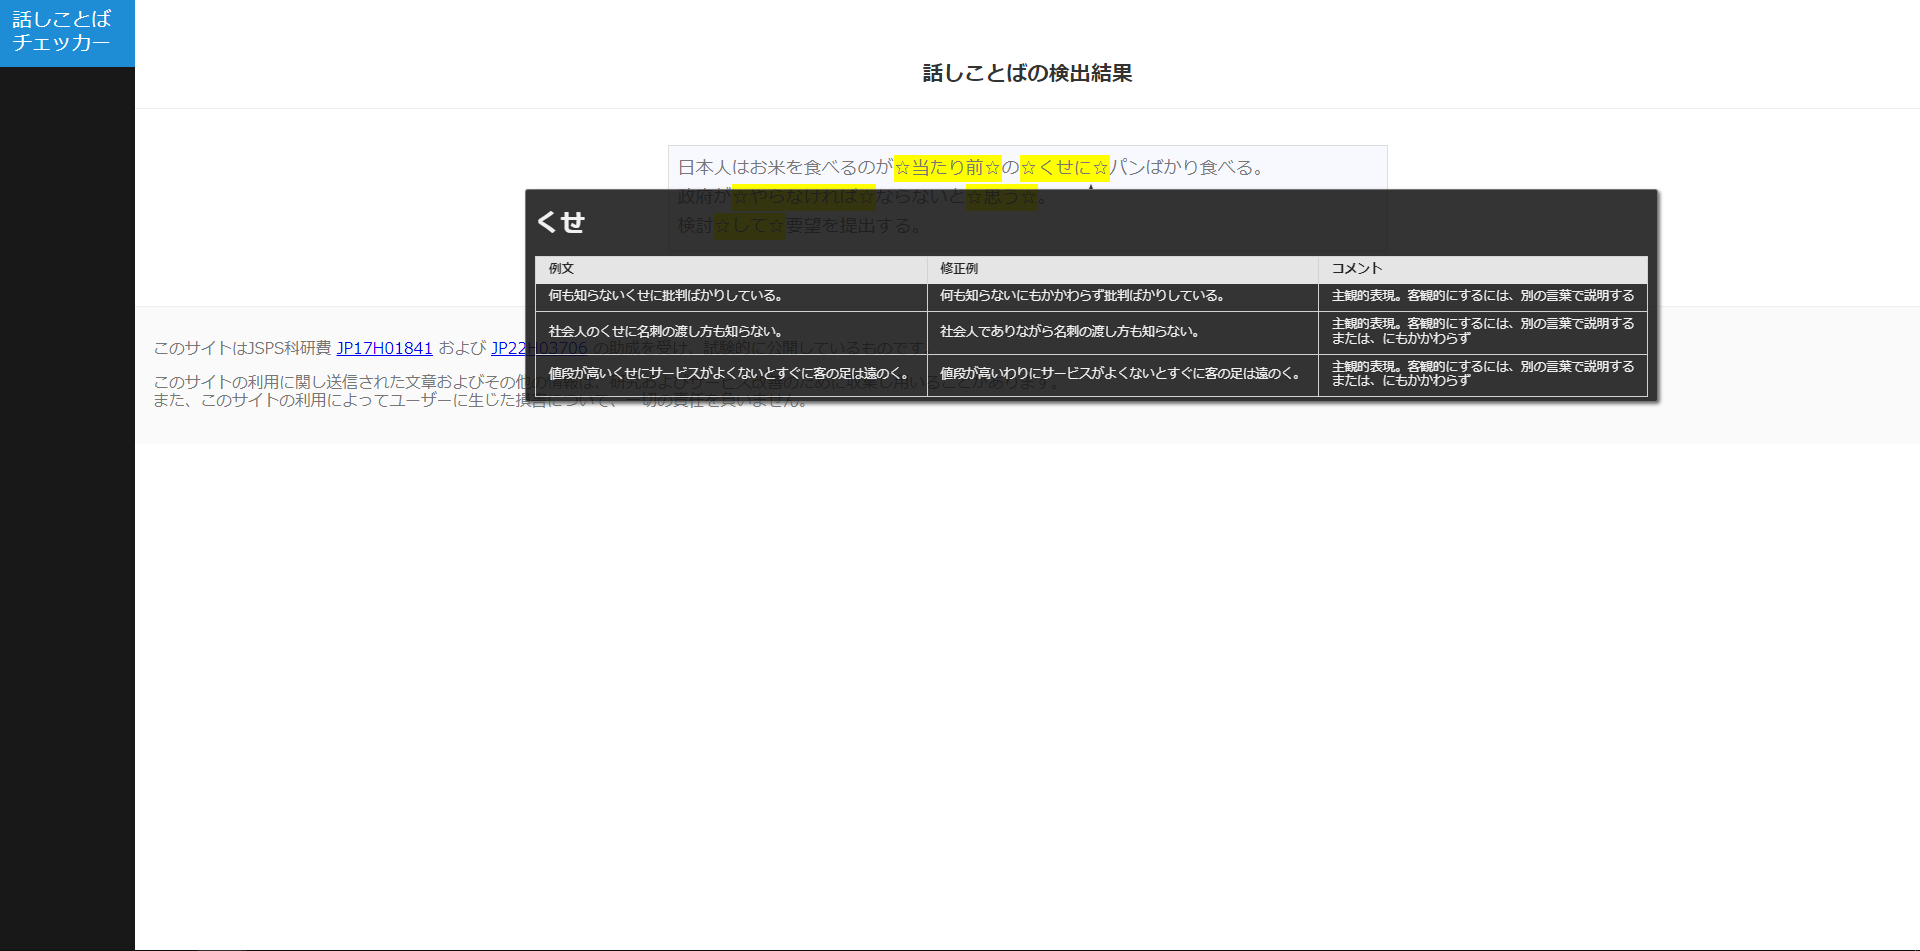
\includegraphics[width=150mm]{image/checkerss-popout.png}
	\caption{修正例などを表示している様子}
	\label{checkerss-popout}
\end{figure}

すべての話しことばのうち,INDEPENDENCE,PREFIX,SUFFIXに振り分けられている話しことばについては,現在運用している話しことばチェッカーで検出可である.一方で,COLLOCATION,OTHERに振り分けられた話しことばは現状では不可能である.COLLOCATIONには,係り受けを伴う「~たり~たり」などの対象単語とそのほかに着目すべき単語との位置が離れているものがある.これは,話しことばの検出方式が対象単語とその前後に隣接する単語をチェックする仕様となっているためである.

現在使用されている話しことばデータベースは,話しことば事例集を基に設計されており\cite{checker-dev},すべての話しことばが上記のカテゴリに分類することができる.しかし,過去の研究において,話しことばであるか書きことばであるかが不明瞭な表現が存在することがわかっており,これらの表現はカテゴリ分類を基にして話しことば検出を行っている本システムでは検出が困難である.本研究チームではこのような表現をグレーゾーンと定義している.

\section{話しことばにおけるグレーゾーン}
レポートに含まれる表現の中には,話しことばであるか書きことばであるかが不明瞭な表現が存在する.
その一例である「~てしまう」という表現は,その表現が現れる文章が主観的な文章であれば話しことばに分類されるが,客観的であれば書きことばに分類される.

例として,「家族に心配をかけたくないため,体調不良でも我慢してしまうことがある.」という文章について,文章内で主語は省略されているが,「私」などの一人称の代名詞が当てはまることが考えられる.この場合は文章が主観的なものとなるため,この「てしまう」は話しことばに分類される.

一方で,「騒がしい場所で話をすると,言葉の聞き違いが多くなってしまう.」といった一般論として述べられている文章の場合は「者」「人間」のような三人称の代名詞が当てはまることが考えられる.この場合は文章が客観的なものとなるため,この「てしまう」は書きことばに分類される.表\ref{ambiguous-ex}にグレーゾーンの例を示す.

\begin{table}[H]
\centering
\caption{グレーゾーンの例}
\begin{tabular}{|l|l|}
\hline
\multicolumn{1}{|c|}{表現} & \multicolumn{1}{c|}{例文} \\ \hline
てしまう   & \begin{tabular}[l]{@{}l@{}}アップライトピアノだと弾いている指が隠れてしまう\end{tabular} \\ \hline
残念      & \begin{tabular}[l]{@{}l@{}}楽しみにしていたイベントが中止になり残念だった\end{tabular} \\ \hline
面倒くさい & \begin{tabular}[l]{@{}l@{}}私生活では話すことを面倒くさがらずに、\\聞かれたことを真摯に答え説明する力をつけるように努力する\end{tabular} \\ \hline
厳しい     & \begin{tabular}[l]{@{}l@{}}ノルマを達成しなければ昇進は厳しい\end{tabular} \\ \hline
感じる     & \begin{tabular}[l]{@{}l@{}}人それぞれ大丈夫と感じることは異なっている\end{tabular} \\ \hline
大切      & \begin{tabular}[l]{@{}l@{}}社会で活躍できる人材を育成することも大切であると考える\end{tabular} \\ \hline
つらい     & \begin{tabular}[l]{@{}l@{}}芸能界は華やかに見えても、肉体的にも精神的にもつらい仕事がある\end{tabular} \\ \hline
\end{tabular}
\label{ambiguous-ex}
\end{table}

% 使用箇所: c3s4

2023年現在は18種類の表現がグレーゾーンに指定されている.本システムでは,グレーゾーンに指定されている特定の表現は一律で話しことばとして検出される状態になっている.表\ref{ambiguous-ex}に現在指定されているグレーゾーンの一覧を示す.

% グレーゾーンの一覧を載せる
 % 話しことばチェッカー
\chapter{機械学習 \label{c4}}
\begin{comment}
機械学習
評価指標
など
\end{comment}

\section{概要\label{c4s1}}
機械学習は,特定のタスクを効率的に処理するため,あるデータが持っているルールやパターンを反復学習を用いて学習し,そこから得られたパターンをもとに予測を行う技術である.2010年代にニューラルネットワークや自然言語処理が登場し,機械学習が再び注目されるようになった.
さらに,ハードウェアの性能の向上およびインターネットの発展により,機械学習に利用できる学習データを容易に収集できるようになったことから,ニューラルネットワークを用いた機械学習が広く用いられるようになった.ニューラルネットワークは,人体の脳の神経細胞であるニューロンおよびそのつながりである神経回路を数理モデルで表現したものである.
ニューラルネットワークが登場する前の機械学習では,データの特徴量などは人間の手によって設定されていたが,特徴量の調整などの調整は機械が自動で行うため,元のデータを与えることで,従来の人間の手による調整よりも高い精度で予測を行うことができる.

機械学習の分野の1つに自然言語処理がある.自然言語とは人間が日常的に使用している言語を指し,これをコンピュータを用いて処理する技術のことである.自然言語処理には大きく4つの段階でテキストデータの処理を行う.

\begin{enumerate}
    \item 形態素解析
    \item 構文解析
    \item 意味解析
    \item 文脈解析
\end{enumerate}

自然言語処理を行う上で,処理の対象となる文書データと,文書に含まれる単語を識別するための辞書が必要となる.自然言語処理分野において課題に挙げられることは,自然言語が本質的に持つ「曖昧さ」が挙げられ,これが文章の解釈が複雑になる要因となっている.これは,単語が持つ意味が複数存在し,その単語が用いられている文章の文脈によって意味が変化するためである.この影響を軽減させるためには,自然言語処理を行うモデルに大量のテキストデータを学習させる必要がある.

\section{二値分類における評価指標 \label{c4s2}}

\subsection{混同行列 \label{c4s2-1}}
機械学習における二値分類の評価指標に,混同行列(Confusion Matrix)がある.二値分類で出力されたクラス分類結果をまとめた行列であり,二値分類タスクを行う機械学習モデルの評価指標として利用される.
 
\begin{figure}[H]
	\centering
	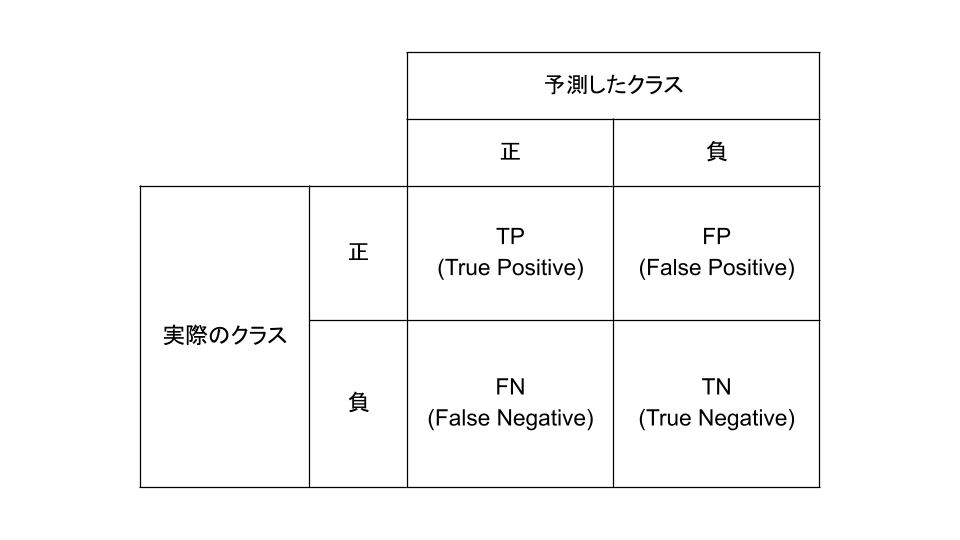
\includegraphics[width=150mm]{image/confusion-matrix.png}
	\caption{混同行列}
	\label{confusion-matrix}
\end{figure}

混同行列左上のTP(True Positive)は,実際のデータが正であるものに対し正と予想されたデータの数である.FP(False Positive)は,実際のデータが正であるものに対し負と予想されたデータである.TN(True Negative)は,実際のデータが負であるものに対し負と予想されたデータである.FN(False Negative)は,実際のデータが負であるものに対し正と予想されたデータの個数である.これら4つの値を用いて,後述する正解率,再現率,適合率,F1値を算出する.

\subsubsection{正解率 \label{c4s2-1a}}
正解率(Accuracy)は,二値分類タスクの評価指標の一つであり,全体の分類結果のうち正答した割合を示す値である.正解率の定義を次式に示す.

$$
\text{Accuracy} = \frac{\text{TP}+\text{FN}}{\text{TP}+\text{TN}+\text{FP}+\text{FN}}
$$


\subsubsection{適合率 \label{c4s2-1b}}
適合率は(Precision)は,二値分類タスクにおける評価指標の一つであり,学習モデルが正と予測したもののうち,実際に正であものの割合を示す値である.適合率の定義を次式に示す.

$$
\text{Precision} = \frac{\text{TP}}{\text{TP}+\text{FP}}
$$

\subsubsection{再現率 \label{c4s2-1c}}
再現率(Recall)は,二値分類タスクの評価指標の一つれあり,実際のデータに含まれる正クラス全体のうち,学習モデルが正と予測したものの割合を示す値である.再現率の定義を次式に示す.

$$
\text{Recall} = \frac{\text{TP}}{\text{TP}+\text{FN}}
$$

\subsubsection{F1値 (F1-score, F-measure) \label{c4s2-1d}}
F1値は,二値分類タスクの一つであり,適合率と再現率の調和平均で算出される値である.適合率と再現率の関係はトレードオフの関係であるため,適合率と再現率の間に差が生じる場合がある.この場合,精度が良いとは一概には判断できない.そのため,これら2つの調和平均を算出し,精度に対し2値のバランスを判断するために用いられる.

$$
\text{F1} = \frac{2 \times \text{Recall} \times \text{Precision}}{\text{Recall}+\text{Precision}}
$$

\section{Attention \label{c4s3}}
Attention は,Transformer の中枢を担う仕組みである.
自然言語処理においては,単語の意味を理解するために,文中のどの単語に注目するすべきかを示すスコアである.Query:${Q}$,Key:${K}$,Value:${V}$の3つのベクトルから計算される.
${K}$と${V}$は1対1の組である.
Attentionは,Self-AttentionとSource-Target-Attentionの2種類がある.また,Attentionの算出方法は加法を使う場合と内積を使う場合があるが,Transformerで使うAttentionは内積を使って算出するため,以降のAttentionの計算は内積を使用していることを前提とする.

\subsection{Self-Attention \label{c4s3-1a}}
${Q}$, ${K}$, ${V}$は全て同じデータから得られた値を使用する.
例として「私/は/大学生/です」という文から${Q}$を得たとすると,${K}$, ${V}$も同じ文から取得する.Transformer では Encoder, Decoder の両方に採用され,文の構造や,形態素同士の関係(例文では「私」=「大学生」)を獲得するために使用される.

\subsection{Target-Attention \label{c4s3-1b}}
${Q}$,${K}$, ${V}$は異なるデータから得られた値を使用する(${K}$, ${V}$は同じデータから取得する).
例として「風邪/を/引いた」,「病院/に/行く」という2文があるとき,${Q}$は「風邪/を/引いた」から,${K}$, ${V}$は「病院/に/行く」から取得する.
 Transfomer では Decoder で採用され,「風邪/を/引いた」→「病院/に/行く」という対話の学習に用いられる.
入力文に対応する出力文が出力されるように学習を行う.

以上の Attention を基本とし,Transformers では Scaled Dot-Product Attention と Multi-Head Attentionが実装されている.
その仕組みを図\ref{mha},図\ref{sda}に示す.

\begin{figure}[H]
	\centering
	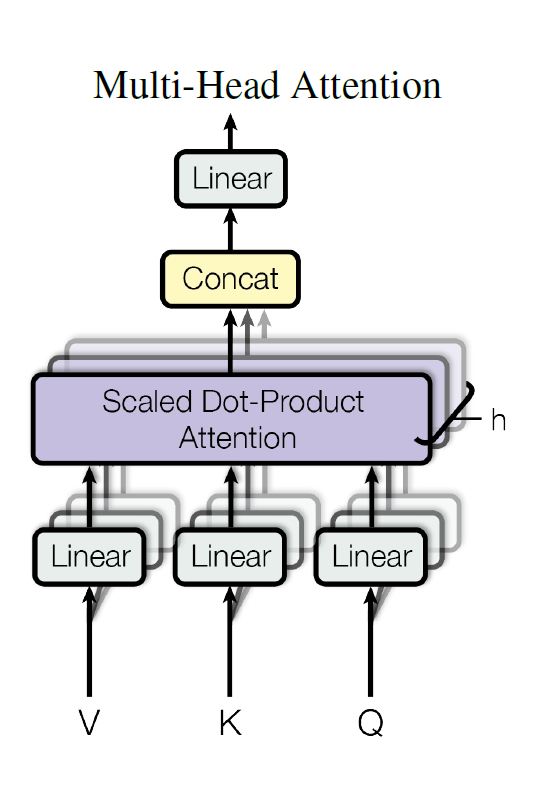
\includegraphics[width=80mm]{image/transformer-multi-head-attention.png}
	\caption{Multi-Head Attentionの構造(\cite{bert}より引用)}
	\label{mha}
\end{figure}

\begin{figure}[H]
	\centering
	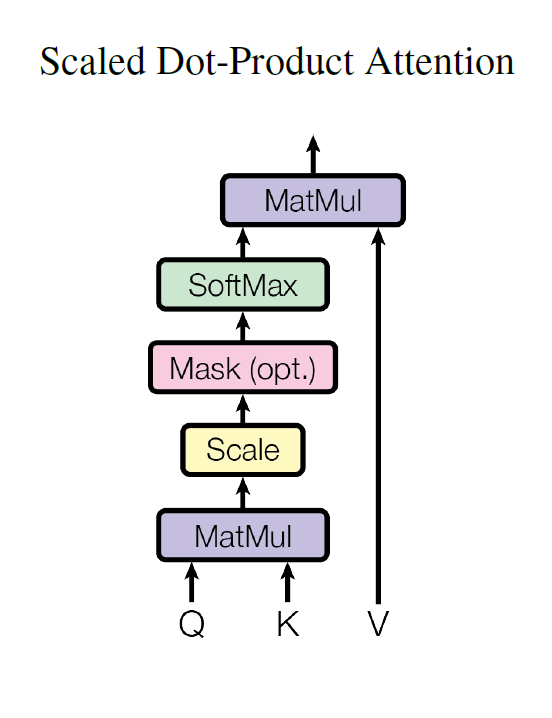
\includegraphics[width=80mm]{image/transformer-scaled-dot-product-attention.png}
	\caption{Scaled Dot-Product Attentionの構造(\cite{bert}より引用)}
	\label{sda}
\end{figure}

\subsubsection{Scaled Dot-Product Attention}
 ${Q}$に対応する${K}$を探し,その${K}$を元にして対応する${V}$を取得する.
まず,${Q}$と${K}$の内積${QK^T}$を取ることで${Q}$に対する${K}$の関連度を算出する.
次に softmax 関数を用いて正規化する.ここで,正規化された値は,Attention の重みであり${Q}$に対応する${K}$の位置を示している.
次に Attention の重みと${V}$の内積を求め,${K}$の位置に対応する${V}$を加重和として取得する.
図 3.5 の数式を式(\ref{attention})に,softmax 関数を式(\ref{softmax})に示す.

\begin{equation}
    \text{Attention}(Q,K,V) = \text{softmax}\left( \frac{QK^T}{\sqrt{d_k}}\right)
    \label{attention}
\end{equation}

\begin{equation}
    \label{softmax}
    \frac{\exp(a_i)}{\sum_{j=1}^{n}\exp(a_j)} \quad(i=1,...,n)
\end{equation}

${QK^T}$の値は次元数に比例して大きくなり,勾配は小さくなってしまう.
そこで式\ref{attention}では${QK^T}$を${\sqrt{d_k}}$で割ることで${QK^T}$の値の増大を防いでいる.
ここで,${d_k}$は${Q}$の次元数を後述する Multi-Head Attention の Head 数で割った値である.

\begin{equation}
    \label{dk}
    d_k = \frac{Q\text{の次元数}}{\text{Multi-Head Attention のHead数}}
\end{equation}

\subsubsection{Multi-Head Attention}
Multi-Head Attention は,Scaled Dot-Product Attention を1つの Head として,複数の Head を並列で処理する仕組みである.
仮に,Head 数が 8 , ${Q}$, ${K}$, ${V}$ の次元数が 512 とすると${\frac{512}{8}=64}$であり,次元数が 64 の ${Q}$, ${K}$, ${V}$ を用いた Scaled Dot-Product Attention を並列に 8 個処理することになる.最終的には個別に計算された値を 1 つのベクトルに落とし込む(concat)ことで単語の分散表現を得る.
この Multi-Head Attention を 1 つのユニット(図 3.2 の Trm )として全結合的に接続したものが BERT モデルである.

\section{Transformer \label{c4s4}}
Transformer とは,再帰型ニューラルネットワーク (以下,RNN) を一切使わずに Attention のみを使うことで,入力と出力の文章同士の広範囲な依存関係を捉えられるモデルである.[7]
RNN は,単語が連続し順序が重要となるような時系列情報を扱うのに最適であるが,逐次的に処理を行うため,処理に多くの時間を必要とする.
また,離れた位置にある文,単語の依存関係をとらえることが難しいといった問題がある.
Transformerは以上のような問題点を克服したモデルである.
Transformerの構造を図\ref{transformer}に示す.

\begin{figure}[H]%3.3
	\centering
	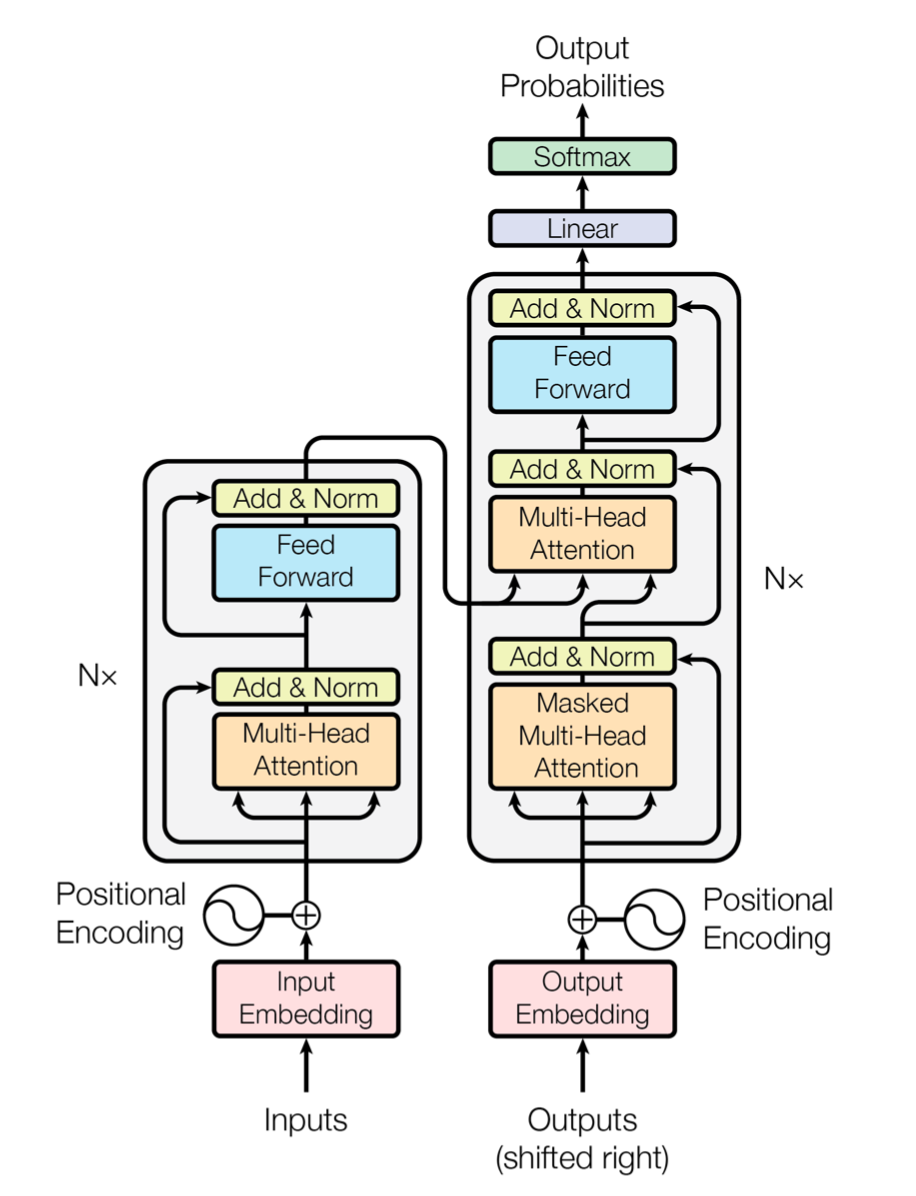
\includegraphics[width=110mm]{image/transformer.png}
	\caption{Transformerの構造(\cite{attention}より引用)}
	\label{transformer}
\end{figure}

\section{BERT \label{c4s5}}
\subsection{概要}
BERT とは,Bidirectional Encoder Representations from Transformers の略で, 「Transformerによる双方向のエンコード表現」と訳され,2018 年に Jacob Devlin らの論文[6] で発表された自然言語処理モデルである.
また,質問応答 (Question Answering) や自然言語推論 (Multi Natural Language Inference) などの 11 種の自然言語処理タスクにおいて当時の最高性能を達成している手法であり,これ以降,このモデルから派生して作られたモデルが多数存在する.また,現在のWeb検索エンジンにも用いられている.

BERT の学習は,大きく2段階に分けられる.
1つ目がラベル付けされていないデータを学習させる「事前学習」であり,2つ目が事前学習時と比較的少量のデータを用いる「Fine Tuning」である.
事前学習で汎用的なモデルを作成し,Fine Tuningを行うことで,個々のタスクに適応したモデルを作成する.

\subsubsection{事前学習}
事前学習は,大量の文章を学習することで,汎用的なモデルを形成する.
ここで得られる事前学習済みモデルをベースとして,この段階より使用するデータの量が少ない「Fine Tuning」を行うことにより,多様なタスクに対応することが可能となる.
BERTは,従来の自然言語処理モデルとは異なり,ラベルが付与されていないデータセットを利用することができる.
これにより,大量のデータを用いることが可能になる.
現状では.自然言語処理タスクのためにラベルが付与されたデータセットが少なく,入手することが困難である.
さらに,ラベルを付与する場合,そのための時間やコストがかかってしまう.
一方,インターネットが普及した現代では,ラベルが付与されていないデータは大量に存在し,容易に入手することが可能である.
そのため,BERTはデータ不足を克服した点で評価されている.
BERTの入力表現を図\ref{input}に示す.

\begin{figure}[H]
	\centering
	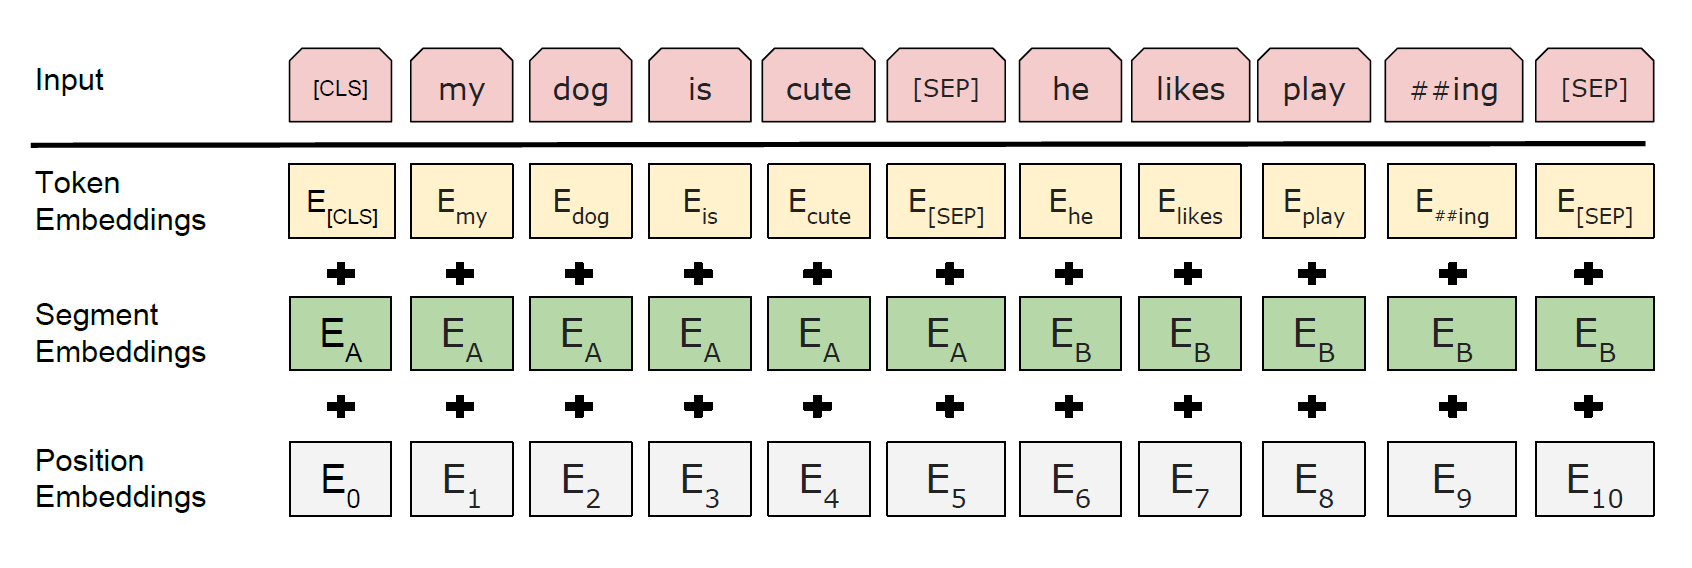
\includegraphics[width=150mm]{image/BERT-input.png}
	\caption{BERTの入力表現}
	\label{input}
\end{figure}

input では,先頭に [CLS] ,文末に [SEP] という特殊なトークンを挿入する.
[CLS] は分類タスクを解く時に使用される (それ以外のタスクではこのトークンは無視される).
[SEP] は文末であることを判別する.
また,入力文の単語数を揃えるために [PAD] トークンを挿入する場合もある.
図 3.6 の Token Embeddings は,input で入力された単語と特殊トークンをIDとして表現している.Segment Embeddings は [SEP] トークンを基準として,1 つ目の文を${E_A}$,2 つ目の文を${E_B}$のように区別した表現,Position Embedding は input 中の単語やトークンの位置を示す表現で,これらの総和が  BERT の入力表現である.

\subsubsection{Masked Language Model}
従来の自然言語処理モデルでは,文章を単一方向からでしか処理できなかった.
そのため,目的の単語より前にある文章データから予測しなければならなかった.
しかし,BERTは双方向のTransformerによって学習するため,従来の手法に比べ精度が向上した.
それを実現しているのが Masked Language Model (以下,MLM) である.入力文の 15 %の単語を確率的に別の token で置き換え,文脈から置き換える前の単語を予測させる.
具体的には,選択された 15 %のうち, 80 %は [MASK] に置き換えるマスク変換,10 %をランダムな異なる単語に変換し,残りの 10 %はそのままの単語にする.

\begin{figure}[H]
	\centering
	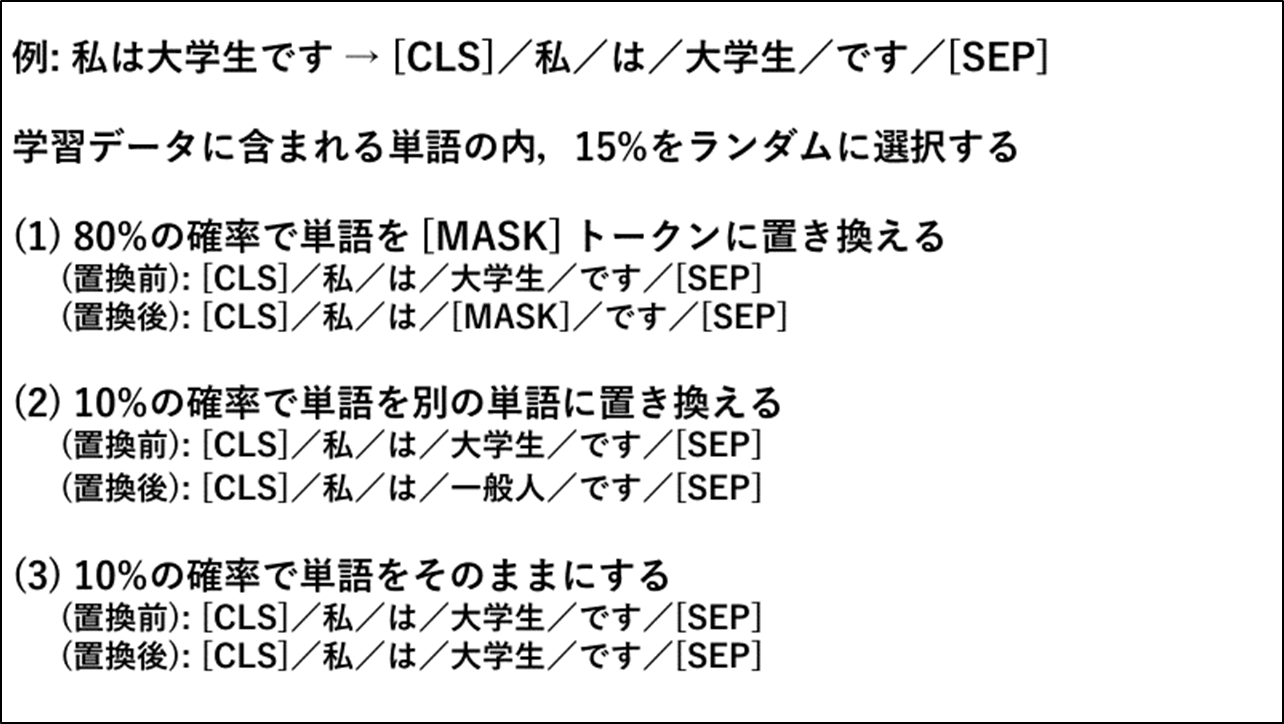
\includegraphics[width=90mm]{image/BERT-mlm.png}
	\caption{Masked Language Model の例}
	\label{mlm}
\end{figure}

\subsubsection{Next Sentence Prediction}
MLM は単語に関しての学習はできるが,文単位の学習はできない.
そこで,2 つの入力文に対して「その 2 文が隣り合っているか」を当てるよう学習する.
これにより,2 つの文の関係性を学習できる.
Next Sentence Prediction (以下,NSP) によって BERT は文章も考慮した,より広範的な自然言語処理モデルとして機能できる.
文の片方を 50 %の確率で他の文に置き換え,それらが隣り合っている(isNext)か隣り合っていない(notNext)か判別することによって学習する.
% NSPの例について画像を載せる
図\ref{nsp}のようなプロセスを大量に繰り返すことで,モデルは言語処理能力を学習する.
本研究では,穴埋め問題を解くことを前提としているため,この処理は行っていない.

\begin{figure}[H]
	\centering
	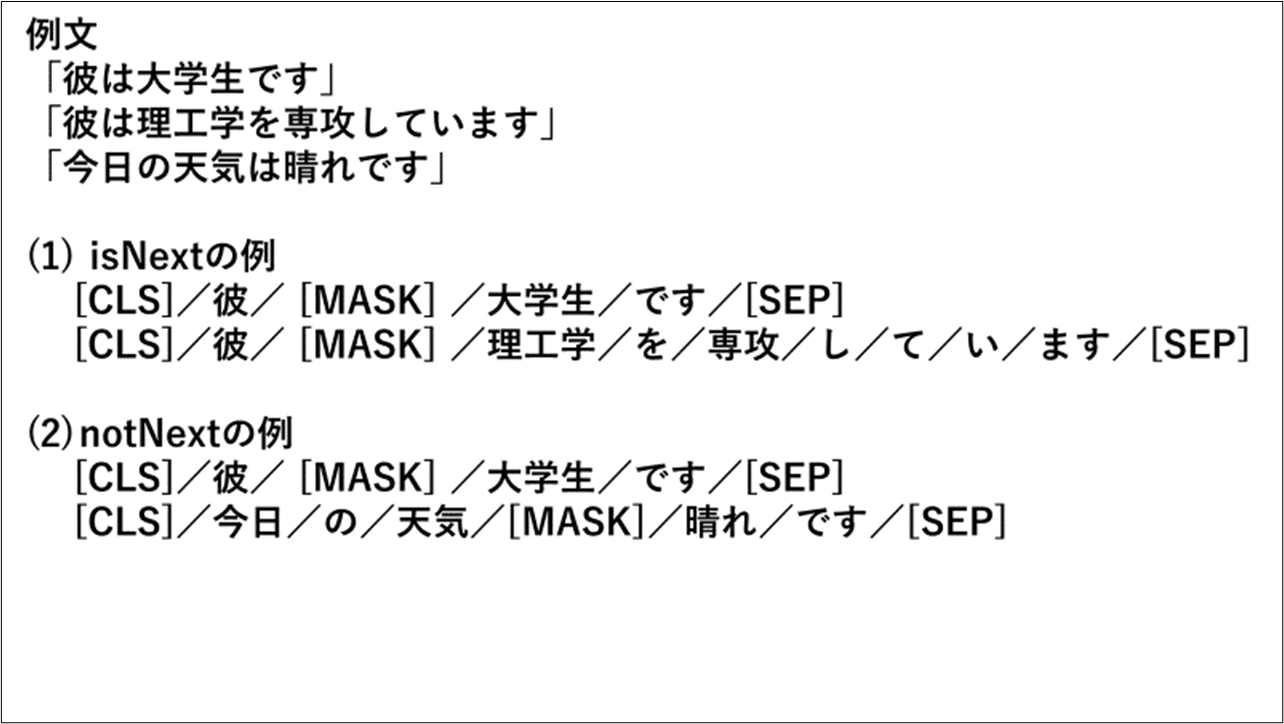
\includegraphics[width=90mm]{image/BERT-nsp.png}
	\caption{NSPの手法}
	\label{nsp}
\end{figure}

\subsubsection{Fine Tuning}
Fine Tuning とは,ある領域の知識を別の領域の学習に適用させる技術である.
従来のタスク処理モデルは特定のタスクにのみ対応している.
しかし,BERT はモデルの構造を修正せずとも,様々なタスクに応用できる.
Pretrained モデルに少量のデータでも Fine Tuning をするだけで重みを 0 から学習するのに比べて,短い時間で学習でき,過学習も抑制することができる.
BERT ではこのような汎用性の高さも評価されている.
図\ref{finetuning}に Fine Tuning の仕組みを示す.
BERT では事前学習で得られたパラメータを初期値として,図\ref{finetuning}のように各タスクごとのレイヤーを上につけて,ラベル付きデータで学習を行う.

\begin{figure}[H]
	\centering
	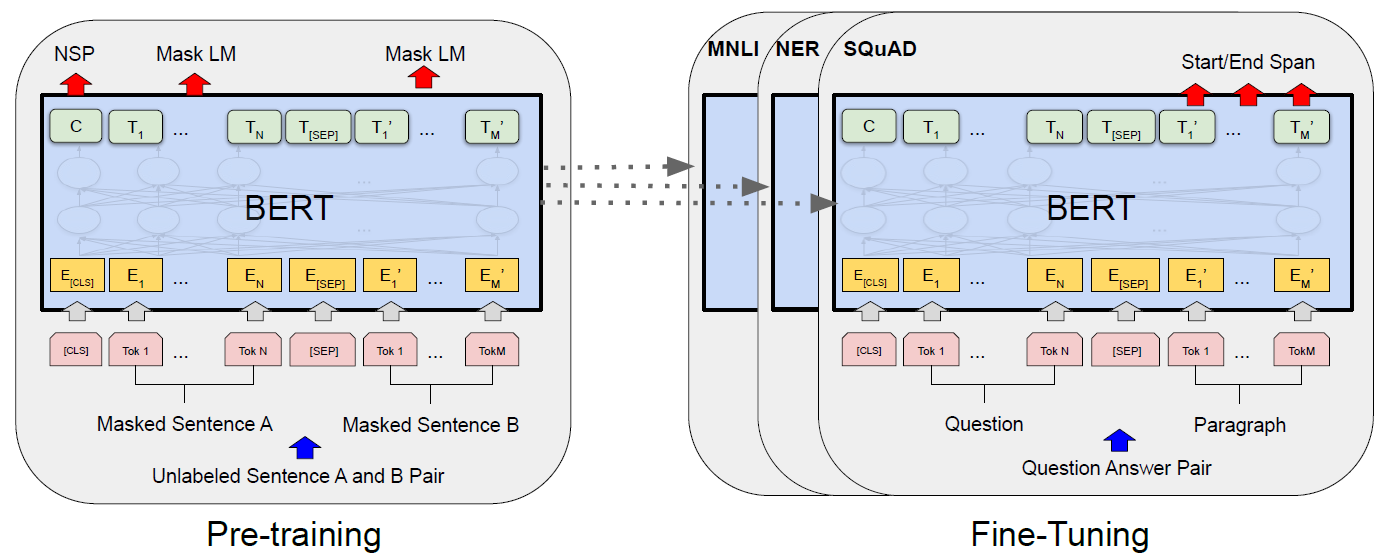
\includegraphics[width=120mm]{image/BERT-finetuning.png}
	\caption{Fine Tuning の仕組み}
	\label{finetuning}
\end{figure}



\section{LLM \label{c4s6}}
LLMとは,Large Language Model の略称であり,大規模言語モデルと呼ばれる.大規模言語モデルという用語についての正式な定義はないが,大規模コーパスを用いて事前学習を行っており,パラメータ総数が数百万以上の言語モデルを指して言われることが多い.LLMの例として,先述のBERTやOpenAI社が開発したChatGPTが挙げられる.

\subsection{ChatGPT}
ChatGPTは,2022年にOpenAI社が発表した対話型の大規模言語モデルである.ユーザが与えた指示(プロンプト)に応じた回答や情報を生成することができる.当時最新であったGPT-3に,

\subsubsection{zero-shot Prompting}
解いてほしいタスクを,具体例を与えずに解かせるプロンプティング手法をZero-shot Promtingという.
% 何かの具体画像を載せる

\subsubsection{one-shot Prompting}
解いてほしいタスクを,具体例を1つだけ与えて解かせるプロンプティング手法をOne-shot Promptingという.
% 何かの具体画像を載せる

\subsubsection{Few-shot Prompting}
解いてほしいタスクを,具体例を複数与えて解かせるプロンプティング手法をFew-shot Promptingという.
% 何かの具体画像を載せる

\section{生成AI \label{c4s7}}
生成AIは,テキストや画像,音声を自律的に生成できるAI技術の総称であり,LLMは生成AIの一部とされる.
生成AIは,文章やテキスト,画像,音声などそれぞれに特化した形で作られている.文章生成であれば先述のGPT-3,GPT-3.5,GPT-4,画像生成であればStable Diffusionが挙げられる.


 % 機械学習
\chapter{事例収集ツールの構築 \label{c5}}

\section{データ収集の課題点の整理 \label{c5s1}}
機械学習モデルを構築するためには,学習に必要なデータの確保や,データにラベルを付与するラベリングの工程が必要となる.しかし,グレーゾーンを含む文章だけを取り出すことやラベリングにおいては,人の手を介して行わなければならない.前述の通り,グレーゾーンは18種類存在し,各々のグレーゾーンを含む文章のみを用意することは現実的とは言い難い.

グレーゾーンの一つである「てしまう」を含む文のデータセットの構築について,専門家への聞き取り調査を行った.質問は以下の2点である.

\begin{enumerate}
    \item 作成期間
    \item 作成方法
\end{enumerate}

作成期間について,専門家からは,「具体的な期間までは記録しておらず,正確な日数までは計算できないが,概ね1か月程度の期間で作成した」と回答していただいた.作成方法については,「基本的には自身が例文を作成しており,インターネット検索を利用し作成した例もある.また,学生レポートから引用している例もある」と回答を頂いたが,このためだけに「てしまう」を含む文を取り出しておらず,専門家が偶然発見したときに引用すると述べていた.

本研究では,上記の聴き取り調査をもとに,学生が執筆したレポートをデータの確保元としてグレーゾーンを含む例文収集の効率化を図った.

\subsection{例文抽出のためのツール構築}
学生のレポートから例文を作成することを想定し,講義内でレポート課題を課してから,レポートの回収・例文の収集,機械学習モデルへの適用までのシミュレートを行った.

\begin{table}[H]
	\centering
        \caption{機械学習モデル適用までの期間の計算}
 	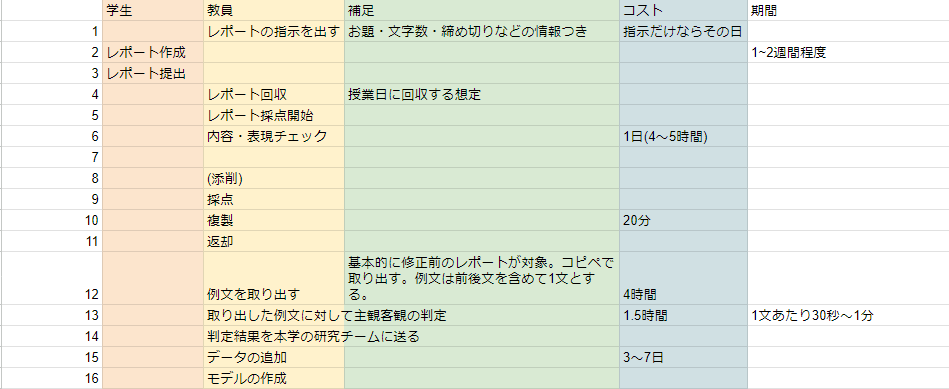
\includegraphics[width=150mm]{image/systemsimurate.png}
	\label{simurate}
\end{table}

以上の工程を整理し,専門的な工程を除けば,例文を取り出す工程が最もコストが高いと考え,本システムとは独立したグレーゾーン表現を含む文章を取り出すツールの構築をおこなった.本ツールは,Python,話しことばチェッカーでも使用されているMeCabを用いて作成しており,グレーゾーンを含む1文および,その前後1文ずつの計3文を抽出している.これは,グレーゾーンを含む文章の主観性・客観性の判定時の補足情報に用いるためである.

\begin{figure}[H]
	\centering
 	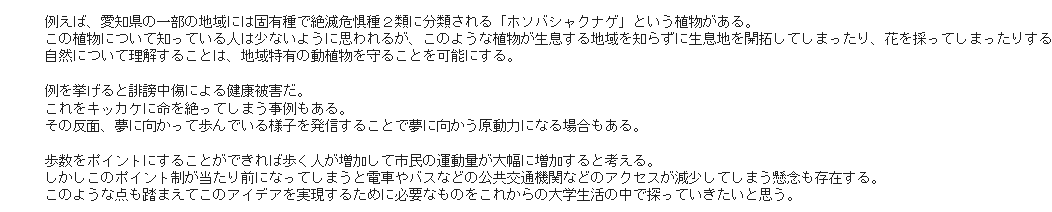
\includegraphics[width=150mm]{image/tool-grayfinder.png}
        \caption{ツールの実行結果}
	\label{grayfinder}
\end{figure}

本ツールにより,成分を取り出す工程の期間の削減が見込められるが,以降の主観性・客観性の判定は,専門家の知識や判断が重要となる.そこで,近年台頭しているLLMの活用を試みた.LLMは対話型の生成AIであり,文脈を読み取れる特性を持つことから,文章の主観性客観性の判断が可能であることが考えられる.グレーゾーンのラベル付けにLLMが活用できると仮定し,グレーゾーン「てしまう」を含む文章の主観客観の判定を通し,ラベル付け工程の代替となり得るかを調査した. % データ収集の課題
\chapter{LLMによるグレーゾーンの主観客観判定 \label{c6}}


\section{LLMによるグレーゾーンの主観客観判定 \label{c6s2}}
LLMは説明不可能なAIであるため,話しことば/書きことばの分類が有効であるかの妥当性を判断することは難しい.そこで,先行研究で使用したBERTモデルによるグレーゾーンを含む文章の主観客観の分類タスクをLLMに行わせた.

本検証では,BERTモデル構築の時に使われた山下が作成したグレーゾーン「てしまう」を含む例文を集めたデータセット475件を用いた.これに対し,以下のようなプロンプトを与え,ChatGPTにグレーゾーンの分類を行わせた.

\begin{table}[H]
\centering
\caption{データセットより抜粋}
\begin{tabular}{|c|l|}
\hline
\multicolumn{1}{|c|}{主観/客観} & \multicolumn{1}{c|}{例文} \\ \hline
主観 & \begin{tabular}[l]{@{}l@{}}以前はゴルフのプレー中にコンタクトが取れてしまうことがあり、\\いつも目のことを気にしていなければならなかった。\end{tabular} \\ \hline
主観 & \begin{tabular}[l]{@{}l@{}}無神経な発言にいちいち腹が立ってしまう自分も大人気ないと思う。\end{tabular} \\ \hline
主観 & \begin{tabular}[l]{@{}l@{}}あせって解約して、思わぬ損をしてしまった。\end{tabular} \\ \hline
主観 & \begin{tabular}[l]{@{}l@{}}言うつもりではなかったのに口をすべらせてしまうことがある。\end{tabular} \\ \hline
客観 & \begin{tabular}[l]{@{}l@{}}絵文字・顔文字は機種間によって表示方法に差異が生じてしまうため、\\自分の感情が正しく受け取る相手に伝えられるとは限らない。\end{tabular} \\ \hline
客観 & \begin{tabular}[l]{@{}l@{}}急いで返信する必要はないと感じると面倒と感じ、特に返信が\\「不必要」と感じたり「催促されている」と感じる際にLINEを使用する\\ことで精神的に疲れを感じてしまうのではないかと考えられる。\end{tabular} \\ \hline
客観 & \begin{tabular}[l]{@{}l@{}}すぐに返信が来ると焦ってしまう、返信する立場のことを考えていない\\ように感じ、余計に返信をする気をなくしてしまうという回答もあった。\end{tabular} \\ \hline
客観 & \begin{tabular}[l]{@{}l@{}}このことにより、返信の催促をされ、受け取った側も精神的に疲れを\\感じLINE使用自体が面倒と感じてしまうようになると考えられる。\end{tabular} \\ \hline
\end{tabular}
\label{ambiguous-sbj-obj}
\end{table}

\subsubsection{検証方法}
プロンプトの構成は,ChatGPTに役割を課す「役割」,取り組んでほしいタスクを示した「指示」,どのようにタスクを取り組むかの例題を記した「例」,出力形式を定めた「フォーマット」,実際に判定してもらう文を記した「判定する文章」の5段で編成した.検証では,「判定する文章」の個数を変えて一度に解かせる量を変化させた場合と,分類時の解答方法を変えた場合で行っている.
また,「例」で使用しているグレーゾーンを含む文章は,データセット構築後新たに追加されたものを使用しており,先行研究\cite{ai-checker}で構築されたBERTモデルの検証データで使われていないものを選択している.

\begin{table}[H]
\centering
\caption{主観客観分類のためのプロンプト(例の組数=3のとき)}
\small % \footnotesize
\begin{tabular}{|l|}
\hline
\multicolumn{1}{|c|}{プロンプト} \\ \hline
\begin{tabular}[c]{@{}l@{}} 
        \#\#\# 役割 \#\#\#\\
        あなた(GPT)を,「大学初年次における日本語文章教育のエキスパート」とします.\\
        \\
        \#\#\# 指示 \#\#\#\\
        「判定する文章」の中の文章それぞれを,主観的であるか客観的であるかを判定してくだ\\さい.\\文章は1文ずつ「。」で区切って提示するので,それぞれについて判定をしてください.\\出力は「フォーマット」に従ってください.「例」では判定理由は省略しています.\\
        <判定理由>は1~2文程度で記述してください.\\
        \\
        \#\#\# 例 \#\#\#\\
        レシートをポケットに入れたまま選択してしまい、洗濯機の掃除に苦労したことがある。\\
        主観的\\
        \\
        風邪を引いてしまい、追試を受けなければならなくなった。\\
        主観的\\
        \\
        病院で処方された薬を飲み忘れてしまったことがある。\\
        主観的\\
        \\
        提出日時に一秒でも遅れてしまうと提出できないようシステム設計されている。\\
        客観的\\
        \\
        Zoomの場合受講生数が多くなると、一画面に収まらなくなり、複数の画面へと分割\\されてしまう。\\
        客観的\\
        \\
        様々な事情により孤独に陥ってしまった人への自治体の支援が十分行き届いていない\\のが現状である。\\
        客観的\\
        \\
        \#\#\# フォーマット \#\#\#\\
        <判定した文章>\\
        <判定結果>\\
        % <判定理由>\\
        \\
        \#\#\# 判定する文章 \#\#\#\\
        「いいね」の数にこだわることは無意味だとはわかっていても、やはり「いいね」の数は\\気になってしまう。\\ \\
        SNSに来たメッセージには「早く返さなければ」と思うため、メッセージを確認する\\ために常にスマホを見てしまうという傾向がある。\\ \\
        スマホ利用実態調査の実験中、「スマホを操作してはならない」という抑圧される\\苦しさに何度も陥ってしまうことがあったが、それでは脱依存を試みることは難しいこと\\も体験した。\\

\end{tabular}   \\ \hline

\end{tabular}
\label{prompt-spokenorwritten}
\end{table}

検証は,以下の項目で行った.
\begin{enumerate}
    \item 主観または客観に分類されている文章を20件ずつ,LLMに主観または客観に分類させる
    \item 主観または客観に分類されている文章を40件ずつ,LLMに主観または客観に分類させる
    \item 主観または客観に分類されている文章を20件ずつ,LLMに話しことばまたは書きことばに分類させる
    \item 主観または客観に分類されている文章を40件ずつ,LLMに話しことばまたは書きことばに分類させる
\end{enumerate}
話しことばまたは書きことばへの分類は,先行研究\cite{checker}の仮定を採用している.

ChatGPTのブラウザ版を使用し,表\ref{prompt-spokenorwritten}と山下が作成したデータセットを40件ずつに分けて回答を生成させたとき,20件ずつに分けて回答を生成させたときのそれぞれで行った.結果の集計は通常の二値分類と同様に,データセットの分類とChatGPTの分類との一致・不一致をそれぞれ集計している.

以上の検証方法を,Zero-shot Prompting, Few-shot Prompting(n=7, 13) の手法で行い,例の組数を変えたことによるChatGPTの回答結果を比較した.ただし,例の組数は話しことば(主観的),書きことば(客観的)の1文ずつ1組として数えている.

\subsection{Zero-shot Promptingでの分類の結果 \label{c6s1-1}}

Zero-shot Promptingでの回答結果の評価を表\ref{cfm-ex0}に示す.各々の条件での混合行列は表\ref{cf-ex0-sw20},表\ref{cf-ex0-sw40},表\ref{cf-ex0-so20},表\ref{cf-ex0-so40}に示す.

\begin{table}[H]
\centering
% \small
\caption{Zero-shot Promptingでの回答結果の評価}
\begin{tabular}{|l|r|r|r|r|}
\hline
\multicolumn{1}{|c|}{} & \multicolumn{1}{c|}{\begin{tabular}[c]{@{}c@{}}話しことば\\書きことば\\ 分類(20件ずつ)\end{tabular}} & \multicolumn{1}{c|}{\begin{tabular}[c]{@{}c@{}}話しことば\\書きことば\\ 分類(40件ずつ)\end{tabular}} & \multicolumn{1}{c|}{\begin{tabular}[c]{@{}c@{}}主観/客観\\ 分類(20件ずつ)\end{tabular}} & \multicolumn{1}{c|}{\begin{tabular}[c]{@{}c@{}}主観/客観\\ 分類(40件ずつ)\end{tabular}} \\ \hline
Accuracy    & 64.26\% & 75.32\% & 64.68\% & 66.26\% \\ \hline
Precision   & 64.63\% & 85.63\% & 65.61\% & 66.26\% \\ \hline
Recall      & 62.98\% & 60.85\% & 61.70\% & 66.26\% \\ \hline
F1          & 63.79\% & 71.14\% & 63.60\% & 66.26\% \\ \hline
\end{tabular}
\label{cfm-ex0}
\end{table}
\begin{table}[H]
\centering
\caption{話しことば/書きことば分類(20件ずつ)の混同行列}
\begin{tabular}{|c|r|r|}
\hline
 & \multicolumn{1}{c|}{\begin{tabular}[c]{@{}c@{}}ChatGPT\\ 書きことば\end{tabular}} & \multicolumn{1}{c|}{\begin{tabular}[c]{@{}c@{}}ChatGPT\\ 話しことば\end{tabular}} \\ \hline
\begin{tabular}[c]{@{}c@{}}山下データセット\\ 書きことば\end{tabular} & 148 & 87 \\ \hline
\begin{tabular}[c]{@{}c@{}}山下データセット\\ 話しことば\end{tabular} & 81 & 154 \\ \hline
\end{tabular}
\label{cf-ex0-sw20}
\end{table}

% 使用箇所: c6s1-1
\begin{table}[H]
\centering
\caption{話しことば/書きことば分類(40件ずつ)の混同行列}
\begin{tabular}{|c|r|r|}
\hline
 & \multicolumn{1}{c|}{\begin{tabular}[c]{@{}c@{}}ChatGPT\\ 書きことば\end{tabular}} & \multicolumn{1}{c|}{\begin{tabular}[c]{@{}c@{}}ChatGPT\\ 話しことば\end{tabular}} \\ \hline
\begin{tabular}[c]{@{}c@{}}山下データセット\\ 書きことば\end{tabular} & 143 & 92 \\ \hline
\begin{tabular}[c]{@{}c@{}}山下データセット\\ 話しことば\end{tabular} & 24 & 211 \\ \hline
\end{tabular}
\label{cf-ex0-sw40}
\end{table}
\begin{table}[H]
\centering
\caption{主観/客観分類(20件ずつ)の混同行列}
\begin{tabular}{|c|r|r|}
\hline
 & \multicolumn{1}{c|}{\begin{tabular}[c]{@{}c@{}}ChatGPT\\ 客観\end{tabular}} & \multicolumn{1}{c|}{\begin{tabular}[c]{@{}c@{}}ChatGPT\\ 主観\end{tabular}} \\ \hline
\begin{tabular}[c]{@{}c@{}}山下データセット\\ 客観\end{tabular} & 145 & 90 \\ \hline
\begin{tabular}[c]{@{}c@{}}山下データセット\\ 主観\end{tabular} & 76 & 159 \\ \hline
\end{tabular}
\label{cf-ex0-so20}
\end{table}
\begin{table}[H]
\centering
\caption{主観/客観分類(40件ずつ)の混同行列}
\begin{tabular}{|c|r|r|}
\hline
 & \multicolumn{1}{c|}{\begin{tabular}[c]{@{}c@{}}ChatGPT\\ 客観\end{tabular}} & \multicolumn{1}{c|}{\begin{tabular}[c]{@{}c@{}}ChatGPT\\ 主観\end{tabular}} \\ \hline
\begin{tabular}[c]{@{}c@{}}山下データセット\\ 客観\end{tabular} & 151 & 84 \\ \hline
\begin{tabular}[c]{@{}c@{}}山下データセット\\ 主観\end{tabular} & 84 & 151 \\ \hline
\end{tabular}
\label{cf-ex0-so40}
\end{table}

話しことば/書きことば分類(40件ずつ)のときのAccuracyが75.32\%で最も高く,適合率も85.63\%と,こちらも最も高い結果が得られた.また,混同行列からは,どの条件においてもPrecisionの数値が高く,話しことば(主観)であるものを正しく判定できる観点での精度が高いことがわかる.

\subsection{考察}
「てしまう」の分類例を与えずにChatGPTに分類をさせたとき,話しことばまたは書きことばとみなして分類させた方が全体の正解率が高くなった.これは,ChatGPTが持つ話しことば・書きことばの認識が主観・客観の認識よりもしやすいことが考えられる.また,一度に分類させる量が多いときの精度が高いことから,分類時に文脈を考慮しながら判定が行えるようになっていることがが考えられる.

\subsection{Few-shot Promptingでの分類の結果(1) \label{c6s1-2}}
例の件数を7件に増やしたときのFew-shot Promptingでの回答結果の評価を表\ref{cfm-ex7}に示す.各々の条件での混合行列は表\ref{cf-ex7-sw20},表\ref{cf-ex7-sw40},表\ref{cf-ex7-so20},表\ref{cf-ex7-so40}に示す.

\begin{table}[H]
\centering
% \small
\caption{Few-shot Promptingでの回答結果の評価}
\begin{tabular}{|l|r|r|r|r|}
\hline
\multicolumn{1}{|c|}{} & \multicolumn{1}{c|}{\begin{tabular}[c]{@{}c@{}}話しことば\\書きことば\\ 分類(20件ずつ)\end{tabular}} & \multicolumn{1}{c|}{\begin{tabular}[c]{@{}c@{}}話しことば\\書きことば\\ 分類(40件ずつ)\end{tabular}} & \multicolumn{1}{c|}{\begin{tabular}[c]{@{}c@{}}主観/客観\\ 分類(20件ずつ)\end{tabular}} & \multicolumn{1}{c|}{\begin{tabular}[c]{@{}c@{}}主観/客観\\ 分類(40件ずつ)\end{tabular}} \\ \hline
Accuracy    & 63.40\% & 67.87\% & 64.04\% & 55.74\% \\ \hline
Precision   & 68.00\% & 75.30\% & 70.63\% & 61.34\% \\ \hline
Recall      & 48.51\% & 53.19\% & 48.09\% & 31.06\% \\ \hline
F1          & 57.22\% & 62.34\% & 57.22\% & 41.24\% \\ \hline
\end{tabular}
\label{cfm-ex7}
\end{table}

% 使用箇所: c6s1-2
\begin{table}[H]
\centering
\caption{話しことば/書きことば分類(20件ずつ)の混同行列}
\begin{tabular}{|c|r|r|}
\hline
 & \multicolumn{1}{c|}{\begin{tabular}[c]{@{}c@{}}ChatGPT\\ 書きことば\end{tabular}} & \multicolumn{1}{c|}{\begin{tabular}[c]{@{}c@{}}ChatGPT\\ 話しことば\end{tabular}} \\ \hline
\begin{tabular}[c]{@{}c@{}}山下データセット\\ 書きことば\end{tabular} & 119 & 116 \\ \hline
\begin{tabular}[c]{@{}c@{}}山下データセット\\ 話しことば\end{tabular} & 56 & 179 \\ \hline
\end{tabular}
\label{cf-ex7-sw20}
\end{table}

% 使用箇所: c6s1-2
\begin{table}[H]
\centering
\caption{話しことば/書きことば分類(20件ずつ)の混同行列}
\begin{tabular}{|c|r|r|}
\hline
 & \multicolumn{1}{c|}{\begin{tabular}[c]{@{}c@{}}ChatGPT\\ 書きことば\end{tabular}} & \multicolumn{1}{c|}{\begin{tabular}[c]{@{}c@{}}ChatGPT\\ 話しことば\end{tabular}} \\ \hline
\begin{tabular}[c]{@{}c@{}}山下データセット\\ 書きことば\end{tabular} & 141 & 94 \\ \hline
\begin{tabular}[c]{@{}c@{}}山下データセット\\ 話しことば\end{tabular} & 19 & 216 \\ \hline
\end{tabular}
\label{cf-ex7-sw40}
\end{table}
\begin{table}[H]
\centering
\caption{主観/客観分類(20件ずつ)の混同行列}
\begin{tabular}{|c|r|r|}
\hline
 & \multicolumn{1}{c|}{\begin{tabular}[c]{@{}c@{}}ChatGPT\\ 客観\end{tabular}} & \multicolumn{1}{c|}{\begin{tabular}[c]{@{}c@{}}ChatGPT\\ 主観\end{tabular}} \\ \hline
\begin{tabular}[c]{@{}c@{}}山下データセット\\ 客観\end{tabular} & 113 & 122 \\ \hline
\begin{tabular}[c]{@{}c@{}}山下データセット\\ 主観\end{tabular} & 47 & 188 \\ \hline
\end{tabular}
\label{cf-ex7-so20}
\end{table}
\begin{table}[H]
\centering
\caption{主観/客観分類(20件ずつ)の混同行列}
\begin{tabular}{|c|r|r|}
\hline
 & \multicolumn{1}{c|}{\begin{tabular}[c]{@{}c@{}}ChatGPT\\ 客観\end{tabular}} & \multicolumn{1}{c|}{\begin{tabular}[c]{@{}c@{}}ChatGPT\\ 主観\end{tabular}} \\ \hline
\begin{tabular}[c]{@{}c@{}}山下データセット\\ 客観\end{tabular} & 73 & 162 \\ \hline
\begin{tabular}[c]{@{}c@{}}山下データセット\\ 主観\end{tabular} & 46 & 189 \\ \hline
\end{tabular}
\label{cf-ex7-so40}
\end{table}

% 使用箇所: c6s1-2

\subsection{考察}
例の数を増やしたが,\ref{c6s1-1}節の結果と大きな変化がないまたはそれよりも低い結果が得られた.混合行列からは話しことば(主観)であるものを正しく判定した個数が多いことから,話しことばの特性がつかみやすいことが考えられる.

\subsection{Few-shot Promptingでの分類の結果(2) \label{c6s1-3}}
例の組数を13件に増やしたときのFew-shot Promptingでの回答結果の評価を表\ref{cfm-ex13}に示す.各々の条件での混合行列は表\ref{cf-ex13-sw20},表\ref{cf-ex13-sw40},表\ref{cf-ex13-so20},表\ref{cf-ex13-so40}に示す.

\begin{table}[H]
\centering
% \small
\caption{Few-shot Promptingでの回答結果の評価(例の組数=13)}
\begin{tabular}{|l|r|r|r|r|}
\hline
\multicolumn{1}{|c|}{} & \multicolumn{1}{c|}{\begin{tabular}[c]{@{}c@{}}話しことば\\書きことば\\ 分類(20件ずつ)\end{tabular}} & \multicolumn{1}{c|}{\begin{tabular}[c]{@{}c@{}}話しことば\\書きことば\\ 分類(40件ずつ)\end{tabular}} & \multicolumn{1}{c|}{\begin{tabular}[c]{@{}c@{}}主観/客観\\ 分類(20件ずつ)\end{tabular}} & \multicolumn{1}{c|}{\begin{tabular}[c]{@{}c@{}}主観/客観\\ 分類(40件ずつ)\end{tabular}} \\ \hline
Accuracy    & 66.17\% & 78.94\% & 65.74\% & 71.70\% \\ \hline
Precision   & 72.62\% & 80.63\% & 74.03\% & 82.28\% \\ \hline
Recall      & 51.91\% & 76.17\% & 48.51\% & 55.32\% \\ \hline
F1          & 60.55\% & 78.34\% & 58.61\% & 66.16\% \\ \hline
\end{tabular}
\label{cfm-ex13}
\end{table}
\begin{table}[H]
\centering
\caption{話しことば/書きことば分類(20件ずつ)の混同行列}
\begin{tabular}{|c|r|r|}
\hline
 & \multicolumn{1}{c|}{\begin{tabular}[c]{@{}c@{}}ChatGPT\\ 書きことば\end{tabular}} & \multicolumn{1}{c|}{\begin{tabular}[c]{@{}c@{}}ChatGPT\\ 話しことば\end{tabular}} \\ \hline
\begin{tabular}[c]{@{}c@{}}山下データセット\\ 書きことば\end{tabular} & 122 & 113 \\ \hline
\begin{tabular}[c]{@{}c@{}}山下データセット\\ 話しことば\end{tabular} & 46 & 189 \\ \hline
\end{tabular}
\label{cf-ex13-sw20}
\end{table}

% 使用箇所: c6s1-3
\begin{table}[H]
\centering
\caption{話しことば/書きことば分類(20件ずつ)の混同行列}
\begin{tabular}{|c|r|r|}
\hline
 & \multicolumn{1}{c|}{\begin{tabular}[c]{@{}c@{}}ChatGPT\\ 書きことば\end{tabular}} & \multicolumn{1}{c|}{\begin{tabular}[c]{@{}c@{}}ChatGPT\\ 話しことば\end{tabular}} \\ \hline
\begin{tabular}[c]{@{}c@{}}山下データセット\\ 書きことば\end{tabular} & 179 & 56 \\ \hline
\begin{tabular}[c]{@{}c@{}}山下データセット\\ 話しことば\end{tabular} & 43 & 192 \\ \hline
\end{tabular}
\label{cf-ex13-sw40}
\end{table}
\begin{table}[H]
\centering
\caption{主観/客観分類(20件ずつ)の混同行列}
\begin{tabular}{|c|r|r|}
\hline
 & \multicolumn{1}{c|}{\begin{tabular}[c]{@{}c@{}}ChatGPT\\ 客観\end{tabular}} & \multicolumn{1}{c|}{\begin{tabular}[c]{@{}c@{}}ChatGPT\\ 主観\end{tabular}} \\ \hline
\begin{tabular}[c]{@{}c@{}}山下データセット\\ 客観\end{tabular} & 114 & 121 \\ \hline
\begin{tabular}[c]{@{}c@{}}山下データセット\\ 主観\end{tabular} & 40 & 195 \\ \hline
\end{tabular}
\label{cf-ex13-so20}
\end{table}

% 使用箇所: c6s1-3
\begin{table}[H]
\centering
\caption{主観/客観分類(40件ずつ)の混同行列}
\begin{tabular}{|c|r|r|}
\hline
 & \multicolumn{1}{c|}{\begin{tabular}[c]{@{}c@{}}ChatGPT\\ 客観\end{tabular}} & \multicolumn{1}{c|}{\begin{tabular}[c]{@{}c@{}}ChatGPT\\ 主観\end{tabular}} \\ \hline
\begin{tabular}[c]{@{}c@{}}山下データセット\\ 客観\end{tabular} & 130 & 105 \\ \hline
\begin{tabular}[c]{@{}c@{}}山下データセット\\ 主観\end{tabular} & 28 & 207 \\ \hline
\end{tabular}
\label{cf-ex13-so40}
\end{table}

% 使用箇所: c6s1-3

\subsection{考察}
例の数をさらに増やしたところ,正解率は\ref{c6s1-1}節よりも高い結果が得られた.これは,例を増やしたことにより,文脈をより正確にとらえられるようになったことが考えられる.また,先行研究\cite{ai-checker}で記録した精度と同等であることから,分類タスクでの応用が考えられる.
一方で,20件ずつ解かせている場合の正解率は\ref{c6s1-1}節とほとんど変化は無かった.これは,前述の通り解かせる量が多く,分類時に文脈を考慮しながら判定が行えるからであると考えられる.

% \subsection{追加検証}
% 一度に解かせる文章が多いと精度が高くなるという結果が得られた.このことより,プロンプトに載せる文章の数によって,精度の向上が期待できる.そこで,話しことば/書きことばへの分類タスクで一度に解かせる量を20件にしているものについて,例の数を追加し,文章の総数を40件の場合と同じ個数,すなわち例33組,分類させる文章20件,計86文をプロンプトに組み込んで分類させた. % LLMと主観客観判定
\chapter{LLMを用いた話しことば検出 \label{c7}}

本章では,LLMを用いた話しことばを検出させる実験について述べる.LLMが持つ話しことばの知識を本システムの話しことばルールを比較し,ChatGPTがもつ話しことばの認識について調査した。

\subsubsection{使用したデータ}
本実験では,2019年度に本学で開講された,2年次が履修する「アルゴリズムとプログラミング」の講義内で提出されたレポートから16件を抽出し,その本文を用いた.後述の各検証では一律でこのデータを用いている.

\subsubsection{検証方法}
検証は,プロンプトに話しことばの検出をせる内容の指示を入力し,得られた出力結果を話しことばチェッカーに通す.このときの出力結果は「話しことばとされたもの」と呼ぶことにし,話しことばチェッカーで検出された話しことばの種類数を精度の指標とし,LLMの話しことばの認識について調査した.

本章の検証では,ChatGPT APIからGPT-4を利用している.表\ref{table-parameter}にAPI使用時のパラメータ設定を示す.

検証時に,話しことばチェッカーで検出した話しことばおよびグレーゾーンの種類を表\ref{result-checker-detect}に示す.

\begin{table}[H]
\caption{API使用時のパラメータ設定}
\label{table-parameter}
\begin{tabular}{|l|l|r|}
\hline
\multicolumn{1}{|c|}{パラメータ名称} & \multicolumn{1}{c|}{説明} & \multicolumn{1}{c|}{値} \\ \hline
Temperature& \begin{tabular}[c]{@{}l@{}}生成する文章のランダム度合を表す.\\ 値が低いほど毎回の出力で同じ生成結果を得やすい.\end{tabular} & 0 \\ \hline
Max\ tokens& 生成する文章の長さを指定する. & 1000 \\ \hline
Frequency penalty & 同じトークンの出やすさを制御する. & 0.4 \\ \hline
\end{tabular}
\end{table}

% 使用箇所: c7
\begin{table}[H]
\centering
\caption{話しことばチェッカーでの検出結果}
\label{result-checker-detect}
\begin{tabular}{|l|r|}
\hline
話しことばの種類 & 20 \\ \hline
グレーゾーン & 2 \\ \hline
\end{tabular}
\end{table}

\section{Few-shot Prompting を用いた話しことば検出 \label{c7s1}}
主観・客観の分類では,文章と分類結果を1組にして,プロンプトに与える例示に組み込んだ.本検証でも同様に,例文とその中に含まれている話しことばを1つの例としてプロンプトに組み込み,話しことば検出を行った.

\begin{table}[H]
\centering
\caption{Few-shot Promptingを用いた話しことば検出のためのプロンプト}
\small % \footnotesize
\begin{tabular}{|l|}
\hline
\multicolumn{1}{|c|}{プロンプト} \\ \hline
\begin{tabular}[c]{@{}l@{}} 
\#\#\# 役割 \#\#\#\\
あなた(GPT)を,「大学初年次における日本語文章教育のエキスパート」\\とします。\\
\\
\#\#\# 指示 \#\#\#\\
与えられた文章から、話しことばである表現を抽出してください。\\
ここでの話しことばの定義は「学術表現として使用することが適切\\ではない表現」です。\\
話しことばを抽出したとき、以下の情報を出力してください。\\
1. 抽出した話しことば\\
\\
\#\#\# 例 \#\#\#\\
Q. 以下の文章から、話しことばである表現を抽出してください。\\
日本人はお米を食べるのが当たり前のくせにパンばかり食べる。\\この件の対応策の策定は政府がやらなければならないとされており、\\政府は検討して要望を提出すると述べている。\\
A. 抽出した話し言葉は以下の通りです。\\
   - 抽出した話しことば1 : 当たり前\\
   - 抽出した話しことば2 : くせに\\
   - 抽出した話しことば3 : やらなければならない\\
   - 抽出した話しことば4 : 検討して\\
\\
Q. 以下の文章から、話しことばである表現を抽出してください。\\
高台の家はあやうく浸水被害を免れた。日頃から防災意識を持つ\\ことの必要性を痛いほど実感した。\\
A. 抽出した話し言葉は以下の通りです。\\
   - 抽出した話しことば1 : あやうく\\
   - 抽出した話しことば2 : くせに\\
\\
(中略)\\
\\
Q. 以下の文章から、話しことばである表現を抽出してください。\\
少子化問題の根本的な解決策はわからない。\\
A. 抽出した話し言葉は以下の通りです。\\
   - 抽出した話しことば1 : わからない
\\
Q. 以下の文章から、話しことばである表現を抽出してください。\\
自ら走ることもあるので\\
A. 抽出した話し言葉は以下の通りです。\\
   - 抽出した話しことば1 : ので\\
\\
\#\#\# 実践 \#\#\# \\
Q. 以下の文章から、話しことばである表現を抽出してください。\\
(レポート本文)
\end{tabular}   \\ \hline
\end{tabular}
\label{prompt-detectspoken-few10}
\end{table}

プロンプトは,LLMが内容を正しく読み取れることを考慮し,LLMに役割を与える「役割」,取り組んでほしいタスクを示した「指示」,「話しことばの具体例」,「書きことばリスト」,「学生のレポート本文(検出をさせる文章)」のように構成した.

本検証では,与える例を0, 2, 5, 10, 40件のときに分けて検証を行った.

\subsection{結果}
LLMの検出結果を表\ref{result-detectspoken-few10}に示す.すべての場合で120種類以上の表現を話しことばとして検出したが,実際に話しことばであったものは,多くても8種類であり,ほとんどすべてが話しことばではない表現であった.

\begin{table}[H]
\caption{Few-shot Promptingを用いたときの検出結果}
\label{result-detectspoken-few10}
\centering
\begin{tabular}{|l|r|r|r|r|r|}
\hline
 & \multicolumn{1}{c|}{zero-shot} & \multicolumn{1}{c|}{\begin{tabular}[c]{@{}c@{}}few-shot\\ 例2件\end{tabular}} & \multicolumn{1}{c|}{\begin{tabular}[c]{@{}c@{}}few-shot\\ 例5件\end{tabular}} & \multicolumn{1}{c|}{\begin{tabular}[c]{@{}c@{}}few-shot(10)\\ 例10件\end{tabular}} & \begin{tabular}[c]{@{}r@{}}話しことば\\ チェッカー\end{tabular} \\ \hline
\begin{tabular}[c]{@{}l@{}}話しことばとして\\ 検出されたもの\\ (単位: 種類)\end{tabular} & 120 & 125 & 135 & 125 & - \\ \hline
\begin{tabular}[c]{@{}l@{}}チェッカーで検出\\ した話しことば\end{tabular} & 6 & 8 & 5 & 5 & 20 \\ \hline
グレーゾーン & 2 & 2 & 2 & 2 & 2 \\ \hline
\begin{tabular}[c]{@{}l@{}}実際は話しことば\\ ではなかったもの\end{tabular} & 106 & 114 & 130 & 118 & - \\ \hline
\end{tabular}
\end{table}

\subsection{考察}
話しことばの検出に焦点を当てていたが,話しことばと対になる存在である書きことばについて言及していないことや,どのようなものが書きことばであるかを理解できていないことが考えられる.これを踏まえ,次節では,書きことばの具体例を新たにプロンプトに組み込んで検証を行った.

\section{書きことばリストを用いた話しことば検出 \label{c7s2}}
明らかに書きことばであると考えられる表現を列挙し,これらの表現を検出しないように指示を加えたプロンプトを用いた検証を行った.
書きことばリストには,誤検出で特に多かった表現を選択している.

\begin{table}[H]
	\centering
        \caption{書きことばリスト}
 	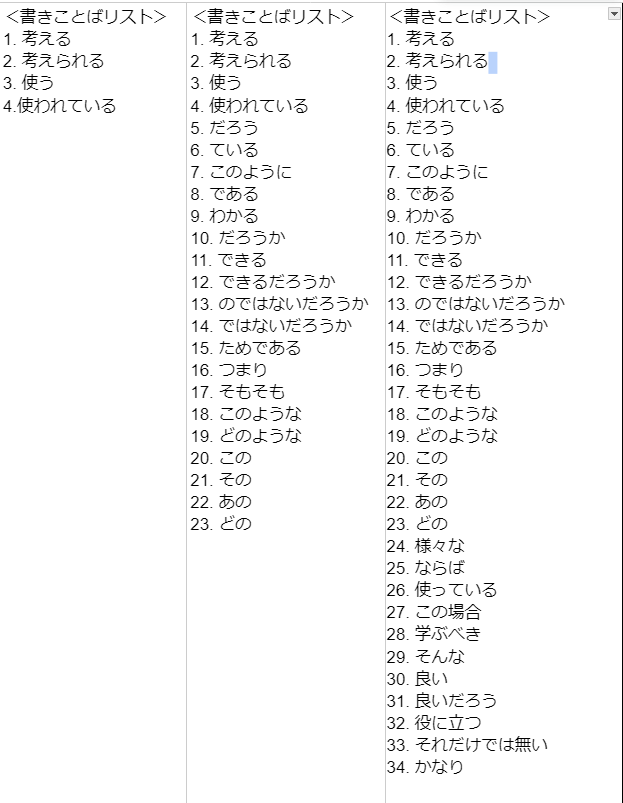
\includegraphics[width=80mm]{image/image-klistTable.png}
	\label{klistTable}
\end{table}

本検証では,\ref{c7s1}節の例40件を与えたときと与えなかったときで比較している.

\subsection{結果}
本検証の結果を表\ref{result-klist-few40},表\ref{result-klist-few0}に示す.例示を入れている方では検出数は70種類以上あるが,実際に話しことばであるものは
\begin{table}[H]
\caption{書きことばリスト組込み時の話しことば検出結果(例あり)}
\label{result-klist-few40}
\centering
\begin{tabular}{|l|r|r|r|}
\hline
\begin{tabular}[c]{@{}l@{}}書きことばリスト\\ の件数\end{tabular} & 4 & 23 & 34 \\ \hline
\begin{tabular}[c]{@{}l@{}}話しことばとして\\ 検出されたもの\\ (単位: 種類)\end{tabular} & 96 & 77 & 90 \\ \hline
\begin{tabular}[c]{@{}l@{}}チェッカーで検出した\\ 話しことば\end{tabular} & 13 & 11 & 12 \\ \hline
グレーゾーン & 2 & 1 & 2 \\ \hline
\begin{tabular}[c]{@{}l@{}}話しことばでは\\ なかったもの\end{tabular} & 81 & 65 & 76 \\ \hline
\end{tabular}
\end{table}
\begin{table}[H]
\caption{書きことばリスト組込み時の話しことば検出結果(例なし)}
\label{result-klist-few0}
\centering
\begin{tabular}{|l|r|r|r|}
\hline
\begin{tabular}[c]{@{}l@{}}書きことばリスト\\ の件数\end{tabular} & 4 & 23 & 34 \\ \hline
\begin{tabular}[c]{@{}l@{}}話しことばとして\\ 検出されたもの\\ (単位: 種類)\end{tabular} & 64 & 58 & 49 \\ \hline
\begin{tabular}[c]{@{}l@{}}チェッカーで検出した\\ 話しことば\end{tabular} & 11 & 10 & 10 \\ \hline
グレーゾーン & 2 & 1 & 2 \\ \hline
\begin{tabular}[c]{@{}l@{}}話しことばでは\\ なかったもの\end{tabular} & 51 & 47 & 37 \\ \hline
\end{tabular}
\end{table}

\subsection{考察}
例を与えたときの方が例を与えなかったときよりも誤検出が多く,検出できた話しことばの種類の数に大きな変化が無く,相対的に検出の精度が低くなることがわかった.このことから,\ref{c7s1}節の方式での例示では話しことば検出の効果が低いことが考えられる.

\section{話しことば・書きことばの定義を変更したときの話しことば検出 \label{c7s3}}
プロンプトには話しことばの定義を記述していたが,LLMが生成した話しことばの定義を利用することで誤検出が減らせると仮定し,LLMに話しことばの定義を生成させ,一部編集を加えたものをプロンプトに組み込み,これを用いて話しことば検出を行った.

\begin{table}[H]
\centering
\caption{プロンプト中の話しことば・書きことばの定義の変更点}
\label{spoken-written-def}
\begin{tabular}{ll}
 & 定義の内容 \\
\begin{tabular}[c]{@{}l@{}}変更前の話しことば・\\ 書きことばの定義\end{tabular} & \begin{tabular}[c]{@{}l@{}}話しことば: 学術表現として使用することが\\ 適切ではない表現\end{tabular} \\
\begin{tabular}[c]{@{}l@{}}変更後の話しことば・\\ 書きことばの定義\end{tabular} & \begin{tabular}[c]{@{}l@{}}書きことば: 公的文書や学術論文、技術文書\\ などで一般的に使用されるフォーマルな表現\\ \\ 話しことば: 日常生活で使う文章や敬語の文章\\ で使用されるインフォーマルな表現\end{tabular}
\end{tabular}
\end{table}

\subsection{結果}

\begin{table}[H]
\centering
\caption{話しことば検出結果}
\label{result-expert}
\begin{tabular}{|l|r|}
\hline
話しことばとして検出されたもの(単位: 種類) & 60 \\ \hline
チェッカーで検出した話しことば & 15 \\ \hline
グレーゾーン & 2 \\ \hline
話しことばではなかったもの & 43 \\ \hline
\end{tabular}
\end{table} % 移行忘れず

\begin{table}[H]
	\centering
        \caption{書きことばリストに載っている表現の出現頻度}
 	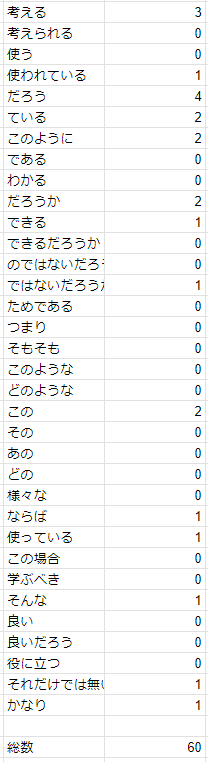
\includegraphics[width=50mm]{image/kenshutu-ichiran-old.png}
	\label{kenshutu-ichiran-old}
\end{table}

\subsection{考察}
書きことばリストを導入したときよりも誤検出が増えた.これは,定義を変更したことにより,定義に沿った検出結果を生成したことが考えられる.

\section{指示を2段階に分けたときの話しことば検出 \label{c7s4}}
書きことばリストにあげられている表現が依然として多いため,得られた出力結果を用いて,書きことばリストに載っている表現を除去するように再度指示を与えた.

\begin{table}[H]
\centering
\caption{話しことば検出のためのプロンプト(後半部)}
\small % \footnotesize
\begin{tabular}{|l|}
\hline
\multicolumn{1}{|c|}{プロンプト} \\ \hline
\begin{tabular}[c]{@{}l@{}} 
\#\#\# 指示 \#\#\# \\
以下の<書きことばリスト>の1から34までの表現は書きことばとします。<書きことばリスト>の言葉が\#\#\# 表現リスト \#\#\#に含まれている場合、\#\#\# 表現リスト \#\#\#から除外して出力してください。
<書きことばリスト>
1. 考える
2. 考えられる
3. 使う
4. 使われている
5. だろう
6. ている
7. このように
8. である
9. わかる
10. だろうか
11. できる
12. できるだろうか
13. のではないだろうか
14. ではないだろうか
15. ためである
16. つまり
17. そもそも
18. このような
19. どのような
20. この
21. その
22. あの
23. どの
24. 様々な
25. ならば
26. 使っている
27. この場合
28. 学ぶべき
29. そんな
30. 良い
31. 良いだろう
32. 役に立つ
33. それだけでは無い
34. かなり

\#\#\# 表現リスト \#\#\# \\
(1度目の出力で得られた「話しことばとされたもの」)
\end{tabular}   \\ \hline

\end{tabular}
\label{prompt-sdetectspoken-klist}
\end{table} % なぜこのプロンプトにしたか書こう

% プロンプトの内容は,表\ref{prompt-detectspoken-api},表\ref{prompt-sdetectspoken-klist}の書きことばリストの部分を抜き取り,\ref{c7s1}節の結果から書きことばリストに当てはまる表現を除去する内容である.

\subsection{結果}
上記のプロンプトで得られた話しことば検出結果を表\ref{kenshutu-ichiran-imp}に示す.

\begin{table}[H]
\centering
\caption{話しことば検出結果}
\label{result-checker-klist2times}
\begin{tabular}{|l|r|}
\hline
話しことばとして検出されたもの(単位: 種類) & 46 \\ \hline
チェッカーで検出した話しことば & 13 \\ \hline
グレーゾーン & 2 \\ \hline
話しことばではなかったもの & 31 \\ \hline
\end{tabular}
\end{table} % 移行忘れず

\begin{table}[H]
	\centering
        \caption{書きことばリストに載っている表現の出現頻度}
 	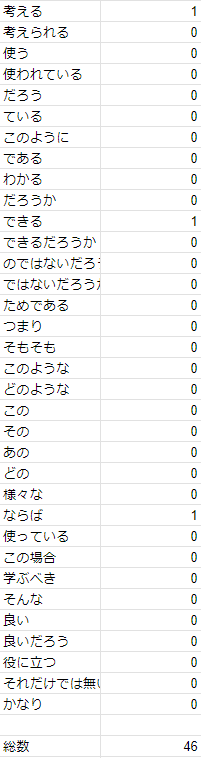
\includegraphics[width=50mm]{image/kenshutu-ichiran-imp.png}
	\label{kenshutu-ichiran-imp}
\end{table}

\subsection{考察}
指示を2段階に分けることにより,書きことばの減少が確認できた.一度の処理では,ChatGPTは最初に書かれた指示を優先して行い,その後の指示を読み取ることが難しいと考えられる.

\section{専門家による判定}
\ref{c7s4}節の結果のうち,話しことばチェッカーで話しことばではないと判定された表現を専門家に判定してもらった.総数は重複を含め21件である.判定項目は(1)話しことばである,(2)グレーゾーン(主観的または客観的),(3)グレーゾーン(判定不能),(4)話しことばではないの4項目である.判定結果を表\ref{bunruikekka}に示す.左列が該当の表現,中央はその表現が含まれている文章,右列は専門家による判定である.

\begin{table}[H]
	\centering
        \caption{専門家の判定結果}
 	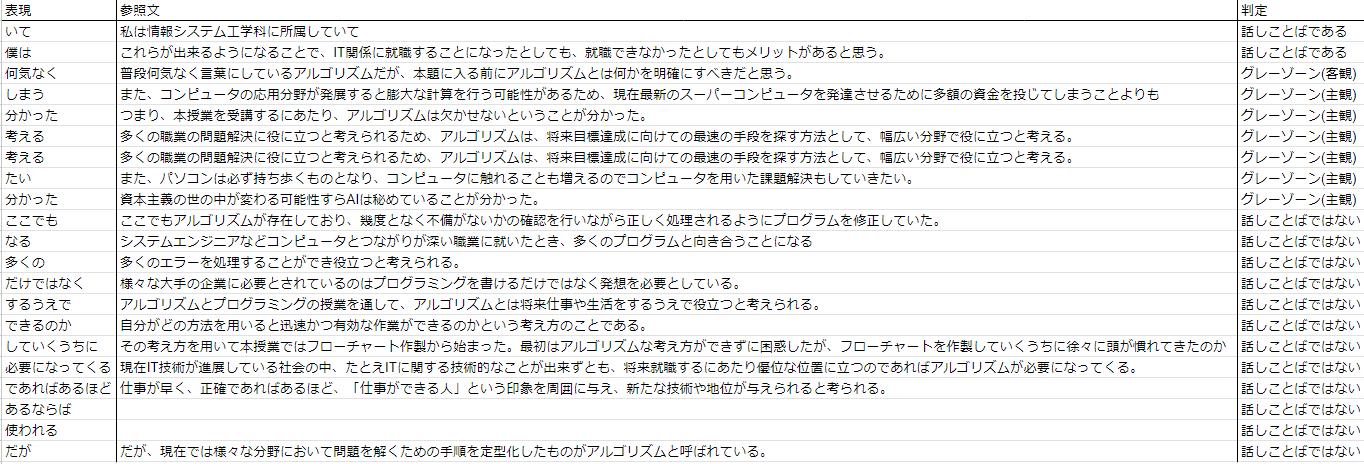
\includegraphics[width=150mm]{image/result-bunruikekka.png}
	\label{bunruikekka}
\end{table}

判定の結果は,話しことばであるものが2件,グレーゾーンであるものが計7件,話しことばではなかったものが12件となり,新規の話しことばが見つかったが,半数は話しことばではない結果となった.

\subsection{考察}
\ref{c7s3}節で使用した定義によって検出された表現のほとんどが話しことばと認められなかった.これについて,LLMはプロンプトに入力した話しことばの定義「日常生活で使う文章や敬語の文章で使用されるインフォーマルな表現」に沿った話しことば検出を行っているが,この定義が本研究チームの話し言葉の定義と異なり,専門家の想定している話しことばと異なる表現を話しことばとして検出したためと考えられる.また,書きことばの定義「公的文書や学術論文、技術文書などで一般的に使用されるフォーマルな表現」としており,書きことばの基準を高く認識している可能性がある. % LLMと話しことば検出
\chapter{結論 \label{c8}}

\section{まとめ}
本研究チームでは,話しことばか書きことばの判断が分かれるグレーゾーン表現に対し,話しことばチェッカーがより柔軟に対応できるようにするため,機械学習と組み合わせたハイブリッドなシステムの構築を目標にあげている.先行研究では,グレーゾーンの1つである「てしまう」に特化した分類モデルを構築したが,機械学習モデル構築時には,大量の学習データや検証データが要求されるうえに,専門家の知識が必要となるラベル付けの工程もあり,「てしまう」以外のグレーゾーンに対応できるようにするには,膨大な労力が必要となる.本研究では,機械学習モデル構築までの工程の整理や,ツールの構築を通した事例収集の効率化を検討し,近年台頭しているLLMを活用したラベル付けの方策を模索した.

検証では,LLMによるグレーゾーンの主観客観分類を行い,先行研究で構築された分類モデルと同等の精度で分類できることがわかり,LLMによるグレーゾーン分類は実用可能性があることが考えられる.

LLMによる話しことば検出では,話しことばの例や,書きことばリストをプロンプトに与えたり,話しことば・書きことばそれぞれの定義を与えることで,LLMでも話しことば検出は可能であることがわかったが,それでも話しことばチェッカーが話しことばと認識しない出力結果もあった.これは,プロンプトに与えた話しことば・書きことばの定義が関係していると考えられ,本研究チームの定義をより具体的なものにして使用すれば,話しことばチェッカーに近い検出が可能になると考えられる.また,専門家の判定では,LLMの検出結果はほとんどグレーゾーンであり,新たな話しことば検出には至れなかったが,前述の通りプロンプトの整備を重ねることで,話しことば検出が可能になると考えられる.

\section{今後の展望}
今後の展望として,LLMによるグレーゾーンの事例文生成が考えられる.本研究では,データ収集の効率化の検討や,LLMによる話しことば検出,先行研究の仮定に基づくグレーゾーンの主観客観判定などの性能調査でとどまっている.今後は,グレーゾーンを含む主観的または客観的な文章の生成を行えるようにプロンプトを整備し,データ収集の効率化が実現できると考えられる.

また,プロンプトに与える話しことばや書きことばの情報をより詳細なものに改良していくことで,話しことばチェッカーと同様の検出が可能になり,入力文を利用した修正が可能になると考えられる.システムでは登録されている修正例を提示していたが,学生が執筆した文章をもとに修正例の提示を行う機能の実装が考えられる.

また,LLMが提示した表現が専門家によって新たな話しことばと認められた場合は,システムの仕様上,話しことばデータベースに登録する必要がある.今後も話しことばとされる表現が変化していくことを想定したシステム運用も検討することが重要であると考えられる.

% しかし,LLMの生成物には事実とは異なる記述が含まれるハルシネーションと呼ばれる現象があり, % 妥当性への脅威
\chapter{結論 \label{c9}}

\section{まとめ \label{c9s1}}
本研究チームでは,話しことばか書きことばの判断が分かれるグレーゾーン表現に対し,話しことばチェッカーがより柔軟に対応できるようにするため,機械学習と組み合わせたハイブリッドなシステムの構築を目標にあげている.先行研究では,グレーゾーンの1つである「てしまう」に特化した分類モデルを構築したが,機械学習モデル構築時には,大量の学習データや検証データが要求されるうえに,専門家の知識が必要となるラベル付けの工程もあり,「てしまう」以外のグレーゾーンに対応できるようにするには,膨大な労力が必要となる.本研究では,機械学習モデル構築までの工程の整理や,ツールの構築を通した事例収集の効率化を検討し,近年台頭しているLLMを活用したラベル付けの方策を模索した.

検証では,LLMによるグレーゾーンの主観客観分類を行い,先行研究で構築された分類モデルと同等の精度で分類できることがわかり,LLMによるグレーゾーン分類は実用可能性があることが考えられる.

LLMによる話しことば検出では,話しことばの例や,書きことばリストをプロンプトに与えたり,話しことば・書きことばそれぞれの定義を与えたりすることで,LLMでも話しことば検出は可能であることがわかったが,それでも話しことばチェッカーが話しことばと認識しない出力結果もあった.これは,プロンプトに与えた話しことば・書きことばの定義が関係していると考えられ,本研究チームの定義をより明確なものにして使用すれば,話しことばチェッカーに近い検出が可能になると考えられる.また,専門家の判定では,LLMの検出結果はほとんどグレーゾーンであり,新たな話しことば検出はわずかしか得られなかったが,前述の通りプロンプトの整備を重ねることで,話しことば検出が可能になると考えられる.

\section{今後の展望 \label{c9s2}}
今後の展望として,\ref{c8s1}節で挙げたような他の条件での検証が考えられる.LLMとしてChatGPT-3.5,GPT-4を使用してきたが,本研究で行った検証では,どちらか片方しか使用していないため,両方で検証を行う必要があると考えられる.また,「てしまう」以外のグレーゾーンでも検証が行えていないため,他のグレーゾーンでも検証が行い,LLMによる主観客観の分類および話しことば検出が有用であるかの見極めができると考えられる.

他には,グレーゾーンの事例文生成が考えられる.本研究では,データ収集の効率化の検討,LLMによる話しことば検出および先行研究の仮定に基づくグレーゾーンの主観客観判定などの性能調査でとどまっている.今後は,グレーゾーンを含む主観的または客観的な文章の生成を行えるようにプロンプトを整備し,データ収集の効率化が実現できると考えられる.

また,プロンプトに与える話しことばや書きことばの情報をより詳細なものに改良していくことで,話しことばチェッカーと同様の検出が可能になり,入力文を利用した修正が可能になると考えられる.システムでは登録されている修正例を提示していたが,学生が執筆した文章をもとに修正例の提示を行う機能の実装が考えられる.

また,LLMが提示した表現が専門家によって新たな話しことばと認められた場合は,システムの仕様上,話しことばデータベースに登録する必要がある.今後も話しことばとされる表現が変化していくことを想定したシステム運用も検討することが重要であると考えられる.

% しかし,LLMの生成物には事実とは異なる記述が含まれるハルシネーションと呼ばれる現象があり, % 結論
\clearpage
\addcontentsline{toc}{chapter}{参考文献} %章立てせずに目次に追加するおまじない
\renewcommand{\bibname}{参考文献} %これがないと,タイトルが「関連図書」になってしまう
\begin{thebibliography}{99999}

\bibitem{checker}
話しことばチェッカーの開発と実証評価, 教育システム情報学会 vol.34 p.99-p.104, 山下由美子,長谷川哲生,山川広人,小松川浩,2020

\bibitem{report-spoken}
学生のレポートにおける話し言葉とその出現傾向, 日本語日本文学 第 28 号 p.57-p.71, 山下由美子,2018

\bibitem{ai-checker}
AI話しことばチェッカーを想定した機械学習モデリングの研究, 川越颯亮, 2023

\bibitem{chatgpt}
ChatGPTブラウザ版,OpenAI,\url{https://chat.openai.com/}


\end{thebibliography}
 % 参考文献
\chapter*{謝辞}

本研究を行うにあたり、主査としてご指導及びご鞭撻をいただきました、公立千歳科学技術大学 小松川 浩 教授に心より感謝申し上げます。学部4年次から3年の間、至らぬ点も多く、多大な迷惑をかけましたが,無事に論文を書き上げることができました。重ねて御礼申し上げます。

副査の公立千歳科学技術大学 萩原 茂樹 教授に深く感謝申し上げます.中間発表では,様々なご助言・ご指摘をしていただき,誠にありがとうございます.

研究を進めていくうえで,様々な相談に乗り,ご指導・ご助言をしていただきました公立千歳科学技術大学 山川 広人 専任講師に深く感謝申し上げます.短い期間でしたが,話しことばチェッカーの開発・運用に携わらせていただきました.本研究のグレーゾーンを含む話しことばの監修をしていただいた帝京大学 山下由美子 講師に深く感謝申し上げます.また,話しことばチェッカー運用に関し多大なご助力をいただいた科研の先生方に感謝申し上げます.

同じ研究チームとしてお世話になった先輩の 川越 颯亮さん,後輩の 須藤 真由 さんに深く感謝申し上げます.お二人に支えられながら研究を進めていくことができました.
大学院の同期として苦楽を共にした西村 貴志さん,新田 大和さん,郡司 凌大さん,三浦 一斗さんに感謝申し上げます.また,日々の生活において,多くのご支援,ご助言をしてくれた両親や,友人の皆さんに感謝の意を表します.

本システムに関する研究は JSPS 科研費 JP17H01841 および JP22H03706 の助成を受けました.本論文を執筆するにあたり,数多くの方々に支えていただいたことに感謝の意を表し,謝辞とさせていただきます. % 謝辞

\end{document}